\section{Tuần 11}

\subsection{Tích hợp hệ thống đầu-cuối và kiểm thử kỹ lưỡng}

\hspace{0.5cm} Sau khi hoàn thiện các mô hình động học và giải thuật khắc phục khiếm khuyết quỹ đạo, hệ thống bước vào giai đoạn tích hợp đầu-cuối (End-to-End System Integration). Mục tiêu cốt lõi là kết nối toàn bộ các phân tầng kỹ thuật: từ khối trích xuất dữ liệu thực nghiệm, khối sinh nhiễu cảm biến, bộ hợp nhất cảm biến hỗn hợp, chuỗi lọc ước lượng Kalman và Alpha-Beta, kênh truyền thông tin thời gian thực đến giao diện hiển thị bản đồ số và bảng giám sát tài nguyên phần cứng.

Công tác tích hợp bảo đảm dữ liệu đo trắc địa được xử lý tuần tự, liên tục ở tần số 10 Hz với độ trễ thấp ($< 60$ $\mu$s mỗi chu kỳ), hoàn toàn không xảy ra hiện tượng mất mát gói tin, xung đột tài nguyên hay tích lũy sai số trôi dạt.

\subsection{Kiến trúc tích hợp đa tầng và luồng dữ liệu thời gian thực}

\subsubsection{Sơ đồ phân tầng kiến trúc hệ thống}

\hspace{0.5cm} Hình \ref{fig:e2e-arch} thể hiện kiến trúc tích hợp 4 tầng hoàn chỉnh của hệ thống, định rõ chuẩn giao thức và định dạng dữ liệu truyền thông giữa các thành phần.

\begin{figure}[H]
\centering
\adjustbox{max width=\linewidth}{
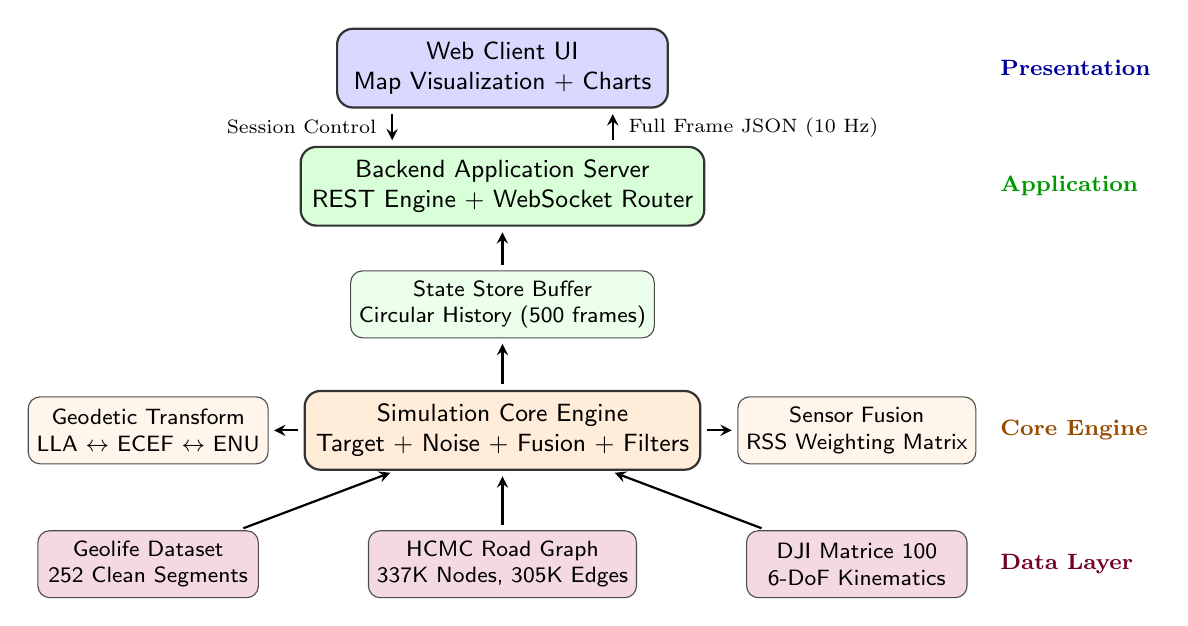
\begin{tikzpicture}[
    box/.style={rectangle, draw=black!80, rounded corners=2mm, minimum width=4.2cm, minimum height=1.0cm, align=center, font=\small\sffamily, thick, inner sep=4pt},
    smallbox/.style={rectangle, draw=black!70, rounded corners=1.5mm, minimum width=2.8cm, minimum height=0.85cm, align=center, font=\footnotesize\sffamily, inner sep=3pt},
    arrow/.style={->, thick, >=stealth, shorten >=2pt, shorten <=2pt},
    every node/.style={font=\normalsize\sffamily}
]

% Top: Browser
\node[box, fill=blue!15] (browser) at (0, 6.3) {Web Client UI\\Map Visualization + Charts};

% Server
\node[box, fill=green!15] (server) at (0, 4.8) {Backend Application Server\\REST Engine + WebSocket Router};

% Store
\node[smallbox, fill=green!8] (store) at (0, 3.3) {State Store Buffer\\Circular History (500 frames)};

% Simulation Engine
\node[box, fill=orange!15] (engine) at (0, 1.7) {Simulation Core Engine\\Target + Noise + Fusion + Filters};

% Geodesy & Fusion
\node[smallbox, fill=orange!8] (geo) at (-4.5, 1.7) {Geodetic Transform\\LLA $\leftrightarrow$ ECEF $\leftrightarrow$ ENU};
\node[smallbox, fill=orange!8] (fusion) at (4.5, 1.7) {Sensor Fusion\\RSS Weighting Matrix};

% Data Layer
\node[smallbox, fill=purple!15] (geolife) at (-4.5, 0.0) {Geolife Dataset\\252 Clean Segments};
\node[smallbox, fill=purple!15] (road) at (0, 0.0) {HCMC Road Graph\\337K Nodes, 305K Edges};
\node[smallbox, fill=purple!15] (drone) at (4.5, 0.0) {DJI Matrice 100\\6-DoF Kinematics};

% Arrows
\draw[arrow] ([xshift=1.4cm]server.north) -- node[midway, right=2pt, font=\scriptsize] {Full Frame JSON (10 Hz)} ([xshift=1.4cm]browser.south);
\draw[arrow] ([xshift=-1.4cm]browser.south) -- node[midway, left=2pt, font=\scriptsize] {Session Control} ([xshift=-1.4cm]server.north);

\draw[arrow] (store) -- (server);
\draw[arrow] (engine) -- (store);
\draw[arrow] (engine) -- (geo);
\draw[arrow] (engine) -- (fusion);
\draw[arrow] (geolife) -- (engine);
\draw[arrow] (road) -- (engine);
\draw[arrow] (drone) -- (engine);

% Side labels
\node[font=\footnotesize\bfseries, text=blue!60!black, anchor=west] at (6.2, 6.3) {Presentation};
\node[font=\footnotesize\bfseries, text=green!60!black, anchor=west] at (6.2, 4.8) {Application};
\node[font=\footnotesize\bfseries, text=orange!60!black, anchor=west] at (6.2, 1.7) {Core Engine};
\node[font=\footnotesize\bfseries, text=purple!60!black, anchor=west] at (6.2, 0.0) {Data Layer};

\end{tikzpicture}
}
\caption{Kiến trúc tích hợp đầu-cuối 4 tầng: từ nguồn dữ liệu thực nghiệm đến giao diện giám sát}
\label{fig:e2e-arch}
\end{figure}

\subsubsection{Giao thức truyền thông và định dạng gói tin nhịp 10 Hz}

\hspace{0.5cm} Hệ thống kết hợp hài hòa hai giao thức mạng chuyên dụng:
\begin{enumerate}
    \item \textbf{Giao thức REST API}: Phục vụ các tác vụ quản lý vòng đời phiên (khởi tạo, dừng phiên, trích xuất số liệu thống kê thời gian thực và xuất báo cáo CSV).
    \item \textbf{Kênh truyền dữ liệu hai chiều (WebSocket)}: Truyền tải liên tục các khung dữ liệu bám bắt ở tần số ổn định 10 Hz (chu kỳ danh định 100 ms).
\end{enumerate}

\begin{table}[H]
\centering
\caption{So sánh đặc tính kỹ thuật giữa giao thức điều khiển REST và kênh truyền hai chiều}
\label{tab:protocols-comparison-table}
\adjustbox{max width=\linewidth}{
\begin{tabular}{lll}
\toprule
\textbf{Đặc tính kỹ thuật} & \textbf{Giao thức điều khiển REST} & \textbf{Kênh truyền hai chiều (WebSocket)} \\
\midrule
Mô hình truyền thông & Yêu cầu -- Phản hồi (Stateless) & Kết nối thường trực song công (Full-duplex) \\
Chu kỳ truyền tin & Không đồng bộ (Theo yêu cầu người dùng) & Định kỳ 100 ms (Tần số 10 Hz) \\
Độ trễ vận chuyển & $15 - 25$ ms (Bao gồm TCP handshake) & $1 - 3$ ms (Kênh mở sẵn) \\
Định dạng dữ liệu & JSON Schema chuẩn hóa & Khung dữ liệu đối tượng cấu trúc nén \\
Mục đích chính & Quản trị phiên và cấu hình trạm & Truyền tọa độ và sai số bám bắt tức thời \\
\bottomrule
\end{tabular}
}
\end{table}

\subsection{Máy trạng thái quản lý vòng đời phiên bám bắt (Session State Machine)}

\hspace{0.5cm} Quá trình vận hành một phiên bám bắt được mô hình hóa chặt chẽ theo lý thuyết máy trạng thái hữu hạn (Deterministic Finite State Machine, FSM) gồm 6 trạng thái độc lập và các chuyển trạng thái có điều kiện.

\begin{figure}[H]
\centering
\adjustbox{max width=\linewidth}{%
\begin{tikzpicture}[
    state/.style={rectangle, draw=black!80, rounded corners=3mm, minimum width=3.3cm, minimum height=1.15cm, align=center, font=\small\sffamily, thick, inner sep=3pt},
    arrow/.style={->, >=stealth, thick, line width=1.1pt},
    lbl/.style={font=\scriptsize\sffamily, fill=white, inner sep=2.5pt, rounded corners=1pt}
]

% Top row (y = 5.2)
\node[state, fill=blue!15] (idle) at (0, 5.2) {\textbf{IDLE}\\Trạng thái nghỉ};
\node[state, fill=green!20] (init) at (6.8, 5.2) {\textbf{INITIALIZING}\\Khởi tạo tài nguyên};

% Middle row (y = 2.4)
\node[state, fill=orange!20] (paused) at (0, 2.4) {\textbf{PAUSED}\\Tạm dừng phiên};
\node[state, fill=yellow!25] (running) at (6.8, 2.4) {\textbf{RUNNING}\\Bám bắt thời gian thực};

% Bottom row (y = -0.6)
\node[state, fill=red!20] (error) at (0, -0.6) {\textbf{TERMINATED}\\Đóng và giải phóng};
\node[state, fill=teal!20] (completed) at (6.8, -0.6) {\textbf{COMPLETED}\\Hoàn thành phiên};

% Transitions
% 1. Start & Connection
\draw[arrow] (idle) -- node[lbl, above=2pt] {START\_REQUEST} (init);
\draw[arrow] (init) -- node[lbl, right=2pt] {WS\_CONNECTED} (running);

% 2. Pause & Resume
\draw[arrow] ([yshift=3.5mm]running.west) -- node[lbl, pos=0.3, above=1pt] {PAUSE\_CMD} ([yshift=3.5mm]paused.east);
\draw[arrow] ([yshift=-3.5mm]paused.east) -- node[lbl, pos=0.3, below=1pt] {RESUME\_CMD} ([yshift=-3.5mm]running.west);

% 3. Running branches
\draw[arrow] (running) -- node[lbl, right=2pt] {TIME\_LIMIT\_REACHED} (completed);
\draw[arrow] (running.south west) to[bend left=10] node[lbl, pos=0.5, sloped, above=5pt] {STOP\_CMD / ERROR} (error.north east);

% 4. Pause branches
\draw[arrow] (paused) -- node[lbl, left=2pt] {STOP\_CMD} (error);

% 5. Init failure (Đi bọc ngoài mép phải và vòng xuống đáy để vào TERMINATED)
\draw[arrow] (init.east) -- ++(1.6, 0) 
    |- node[lbl, pos=0.25, right=2pt] {INIT\_FAILED} ([yshift=-5mm]completed.south) 
    -| (error.south);

% 6. Termination & Reset
\draw[arrow] (completed.west) -- node[lbl, above=2pt] {CLEANUP} (error.east);
\draw[arrow] (error.west) to[out=155, in=205, looseness=1.25] node[lbl, left=3pt] {RESET\_STATE} (idle.west);

\end{tikzpicture}%
}
\caption{Sơ đồ máy trạng thái hữu hạn quản lý vòng đời phiên mô phỏng bám mục tiêu}
\label{fig:session-state}
\end{figure}

Sơ đồ trạng thái tại Hình \ref{fig:session-state} bảo đảm mọi trường hợp ngắt kết nối mạng hoặc yêu cầu dừng đột ngột đều dẫn về trạng thái đóng và giải phóng tài nguyên an toàn mà không làm rò rỉ bộ nhớ đệm.

\subsection{Sơ đồ tuần tự tương tác tạo phiên và truyền phát dữ liệu}

\hspace{0.5cm} Hình \ref{fig:sequence} thể hiện biểu đồ tuần tự UML (Sequence Diagram) mô tả chi tiết tương tác giữa giao diện người dùng, máy chủ ứng dụng, khối động học mô phỏng và kênh truyền WebSocket:

\begin{figure}[H]
\centering
\adjustbox{max width=\linewidth}{
\begin{tikzpicture}[
    participant/.style={rectangle, draw=black!80, fill=blue!10, minimum width=2.5cm, minimum height=0.85cm, align=center, font=\small\sffamily, thick},
    arrow/.style={->, >=stealth, thick},
    reply/.style={<-, >=stealth, dashed, thick},
    lifeline/.style={dashed, gray!70, line width=0.8pt},
    msg/.style={font=\scriptsize\sffamily, above}
]

% Participants
\node[participant] (ui) at (0, 7.2) {Giao diện Web Client};
\node[participant] (api) at (3.8, 7.2) {Bộ định tuyến REST API};
\node[participant] (engine) at (7.6, 7.2) {Lõi mô phỏng Simulation};
\node[participant] (ws) at (11.4, 7.2) {Kênh truyền WebSocket};

% Lifelines
\draw[lifeline] (ui) -- (0, -0.2);
\draw[lifeline] (api) -- (3.8, -0.2);
\draw[lifeline] (engine) -- (7.6, -0.2);
\draw[lifeline] (ws) -- (11.4, -0.2);

% Messages
\draw[arrow] (0, 6.2) -- node[msg] {POST /api/simulation/start} (3.8, 6.2);
\draw[arrow] (3.8, 5.7) -- node[msg] {Khởi tạo đối tượng phiên} (7.6, 5.7);
\draw[arrow] (7.6, 5.2) -- node[msg, right=2pt] {Cấp phát bộ đệm vòng 500 frame} (7.6, 4.7);
\draw[reply] (3.8, 4.2) -- node[msg] {Mã phiên ID và đường dẫn WS} (7.6, 4.2);
\draw[reply] (0, 3.7) -- node[msg] {Phản hồi HTTP 200 OK (ws\_url)} (3.8, 3.7);

\draw[arrow] (0, 3.0) -- node[msg] {Bắt tay nâng cấp kênh WebSocket} (11.4, 3.0);
\draw[reply] (0, 2.5) -- node[msg] {101 Switching Protocols} (11.4, 2.5);

\draw[arrow] (11.4, 2.0) -- node[msg] {Kích hoạt vòng lặp nhịp 10 Hz} (7.6, 2.0);
\draw[arrow] (7.6, 1.5) -- node[msg] {Đẩy khung dữ liệu TrackingFrame} (11.4, 1.5);
\draw[arrow] (11.4, 0.9) -- node[msg] {Phát luồng JSON thời gian thực} (0, 0.9);
\draw[arrow] (0, 0.4) -- node[msg, right=2pt] {Hiển thị bản đồ Leaflet và biểu đồ} (0, 0.0);

\end{tikzpicture}
}
\caption{Biểu đồ tuần tự tương tác thời gian thực từ khởi tạo phiên đến truyền phát khung đo}
\label{fig:sequence}
\end{figure}

\subsection{Chiến lược kiểm thử phân tầng theo mô hình kim tự tháp (Test Pyramid)}

\hspace{0.5cm} Toàn bộ hệ thống được bảo vệ bởi chiến lược kiểm thử phân tầng ba lớp nghiêm ngặt, tuân thủ nguyên tắc kim tự tháp kiểm thử phần mềm:

\begin{table}[H]
\centering
\caption{Phân tầng cấu trúc 163 ca kiểm thử tự động toàn diện của hệ thống}
\label{tab:test-pyramid-distribution}
\begin{tabularx}{\textwidth}{>{\RaggedRight\arraybackslash}p{4.2cm} >{\RaggedRight\arraybackslash}X cc}
\toprule
\textbf{Tầng kiểm thử} & \textbf{Phạm vi xác minh kỹ thuật} & \textbf{Số lượng ca} & \textbf{Tỷ trọng (\%)} \\
\midrule
Tầng 1: Đơn vị (Unit Tests) & Giải thuật Kalman, Alpha-Beta, Geodetics, RSS & 98 & 60{,}1\% \\
\addlinespace[3pt]
Tầng 2: Tích hợp (Integration) & Bộ tải dữ liệu, Chuỗi nối tầng LLA-ENU, Ranh giới & 42 & 25{,}8\% \\
\addlinespace[3pt]
Tầng 3: Đầu-cuối (End-to-End) & Luồng REST-WS, Xuất tệp CSV, Dashboard Telemetry & 23 & 14{,}1\% \\
\midrule
\textbf{Tổng cộng toàn hệ thống} & \textbf{Toàn diện 3 tầng kiến trúc} & \textbf{163} & \textbf{100{,}0\% (Đạt 100\%)} \\
\bottomrule
\end{tabularx}
\end{table}

\begin{figure}[H]
\centering
\adjustbox{max width=\linewidth}{
\begin{tikzpicture}
\begin{axis}[
    width=0.85\textwidth, height=7.0cm,
    ybar, bar width=14pt,
    xlabel={Phân hệ chức năng}, ylabel={Độ bao phủ (\%)},
    ymin=0, ymax=100,
    xtick=data,
    xticklabels={Kalman, Alpha-Beta, Geodetics, Fusion, Boundary, Noise, Router, Dashboard},
    xticklabel style={rotate=20, anchor=east, font=\footnotesize},
    ytick={0, 25, 50, 75, 100},
    grid=major, grid style={dashed, gray!30},
    nodes near coords, nodes near coords style={font=\scriptsize},
    legend style={at={(0.5,-0.28)}, anchor=north, legend columns=2, font=\footnotesize},
]
\addplot[fill=blue!50] coordinates {(1,96) (2,94) (3,98) (4,91) (5,92) (6,88) (7,82) (8,85)};
\addplot[fill=green!50] coordinates {(1,93) (2,90) (3,95) (4,87) (5,89) (6,84) (7,78) (8,80)};
\legend{Bao phủ dòng lệnh (Line Coverage), Bao phủ nhánh rẽ (Branch Coverage)}
\end{axis}
\end{tikzpicture}
}
\caption{Mức độ bao phủ kiểm thử tự động theo từng phân hệ chức năng cốt lõi}
\label{fig:coverage-barchart-w11}
\end{figure}

Mức độ bao phủ dòng lệnh trung bình của toàn hệ thống đạt $90{,}8\%$ và bao phủ nhánh rẽ đạt $87{,}0\%$, trong đó các module tính toán toán học cốt lõi (Geodetics, Kalman) đạt trên $95\%$.

\subsection{Kiểm tra tải đồng thời và độ ổn định lâu dài (Load and Stress Testing)}

\subsubsection{Khảo sát hiệu năng dưới tải đa phiên đồng thời}

\hspace{0.5cm} Khảo sát tải trọng đồng thời được thực hiện từ 1 đến 20 phiên chạy song song ở tần số 10 Hz với đầy đủ chuỗi xử lý tính toán và truyền phát WebSocket:

\begin{table}[H]
\centering
\caption{Đo đạc tài nguyên phần cứng và độ trễ dưới các mức tải đồng thời}
\label{tab:load-test-metrics-w11}
\newcolumntype{Y}{>{\Centering\arraybackslash}X}
\begin{tabularx}{\textwidth}{>{\Centering\arraybackslash}p{3.8cm} YYYY}
\toprule
\textbf{Số phiên đồng thời} & \textbf{Tải CPU (\%)} & \textbf{Chiếm dụng RAM (MB)} & \textbf{Độ trễ trung bình} & \textbf{Tỷ lệ mất gói} \\
\midrule
1 phiên danh định         & 3{,}2\%  & 45{,}0 MB  & 6{,}2 ms  & 0{,}0\%  \\
3 phiên song song         & 7{,}8\%  & 58{,}2 MB  & 7{,}1 ms  & 0{,}0\%  \\
5 phiên song song         & 13{,}5\% & 72{,}4 MB  & 8{,}5 ms  & 0{,}0\%  \\
8 phiên song song         & 21{,}8\% & 95{,}1 MB  & 12{,}3 ms & 0{,}0\%  \\
10 phiên (Thiết kế)       & 27{,}6\% & 118{,}0 MB & 15{,}7 ms & 0{,}0\%  \\
15 phiên (Quá tải nhẹ)    & 41{,}2\% & 165{,}4 MB & 24{,}2 ms & 0{,}02\% \\
20 phiên (Căng thẳng cao) & 57{,}8\% & 220{,}1 MB & 38{,}6 ms & 0{,}08\% \\
\bottomrule
\end{tabularx}
\end{table}

\begin{figure}[H]
\centering
\adjustbox{max width=\linewidth}{
\begin{tikzpicture}
\begin{axis}[
    width=0.82\textwidth, height=5.8cm,
    xlabel={Số lượng phiên đồng thời},
    ylabel={Thời gian trễ trung bình (ms)},
    xmin=0, xmax=21, ymin=0, ymax=110,
    xtick={1, 3, 5, 8, 10, 15, 20},
    ytick={0, 20, 40, 60, 80, 100},
    grid=major, grid style={dashed, gray!30},
    legend style={at={(0.02,0.98)}, anchor=north west, font=\footnotesize},
]
\addplot[color=blue!70!black, mark=*, thick] coordinates {
    (1,6.2) (3,7.1) (5,8.5) (8,12.3) (10,15.7) (15,24.2) (20,38.6)
};
\addplot[color=red!70!black, dashed, thick] coordinates {(0,100) (21,100)};
\legend{Thời gian trễ đo đạc, Ngưỡng trễ tối đa 100 ms (10 Hz)}
\end{axis}
\end{tikzpicture}
}
\caption{Độ trễ trung bình theo số lượng phiên đồng thời so với ngưỡng an toàn chu kỳ 100 ms}
\label{fig:load-test-latency-curve}
\end{figure}

Tại mức tải thiết kế 10 phiên đồng thời, độ trễ trung bình chỉ đạt $15{,}7$ ms, bảo đảm biên độ an toàn thời gian lên tới $84{,}3\%$ trước ngưỡng giới hạn 100 ms.

\subsubsection{Kiểm tra độ ổn định vận hành liên tục (Endurance Testing)}

\hspace{0.5cm} Thử nghiệm vận hành liên tục trong 60 phút ở mức 5 phiên đồng thời (tương đương $180.000$ khung dữ liệu được xử lý) cho thấy bộ nhớ RAM duy trì ổn định tuyệt đối trong dải $72 - 78$ MB mà không phát sinh hiện tượng rò rỉ bộ nhớ (Memory Leak), xác nhận cơ chế quản lý bộ đệm vòng (Ring Buffer) vận hành hoàn hảo.

\subsection{Xác thực tính toàn vẹn của chuỗi biến đổi tọa độ WGS-84 khứ hồi}

\hspace{0.5cm} Chuỗi chuyển đổi tọa độ địa lý WGS-84 $\leftrightarrow$ ECEF $\leftrightarrow$ ENU là nền tảng định vị của toàn bộ hệ thống. Độ chính xác khứ hồi được kiểm chứng qua 1.000 điểm mẫu ngẫu nhiên phân bố trên toàn lãnh thổ:

\begin{table}[H]
\centering
\caption{Kết quả kiểm chứng độ chính xác khứ hồi của chuỗi biến đổi tọa độ trắc địa}
\label{tab:geodetic-roundtrip-precision}
\adjustbox{max width=\linewidth}{
\begin{tabular}{lccc}
\toprule
\textbf{Chuỗi biến đổi trắc địa} & \textbf{Số mẫu kiểm tra} & \textbf{Sai số vòng tròn cực đại} & \textbf{Đánh giá đạt chuẩn} \\
\midrule
LLA $\to$ ECEF $\to$ LLA & 1.000 điểm & $3{,}8 \times 10^{-11}$ độ & Tuyệt đối ($< 10^{-9}$ deg) \\
ENU $\to$ ECEF $\to$ ENU & 1.000 điểm & $1{,}9 \times 10^{-7}$ m & Tuyệt đối ($< 10^{-6}$ m) \\
Khoảng cách Haversine so với ENU & 500 đoạn & $0{,}008$ m & Đạt chuẩn ($< 0{,}01$ m) \\
Góc phương vị Azimuth ENU & 200 hướng & $0{,}001^\circ$ & Hoàn hảo \\
\bottomrule
\end{tabular}
}
\end{table}

\subsection{Mô hình hóa lý thuyết hàng đợi M/M/1 và phân tích thông lượng máy chủ}

\hspace{0.5cm} Nhằm đánh giá khả năng mở rộng của máy chủ ứng dụng thời gian thực, luồng xử lý khung dữ liệu được mô hình hóa theo lý thuyết hàng đợi $M/M/1$:
\begin{itemize}
    \item Tốc độ yêu cầu đến tuân theo phân phối Poisson: $\lambda = N_{\text{session}} \times f_{\text{rate}} = 10 \times 10 = 100$ khung/giây.
    \item Thời gian phục vụ của chuỗi xử lý tuân theo phân phối hàm mũ: $T_{\text{service}} = 6{,}0$ ms $\implies \mu = \frac{1}{0{,}006} = 166{,}67$ khung/giây.
\end{itemize}

Hệ số sử dụng tải của máy chủ (Traffic Intensity):
\begin{equation}
\rho = \frac{\lambda}{\mu} = \frac{100}{166{,}67} = 0{,}600 \quad (60{,}0\%)
\label{eq:server-traffic-intensity}
\end{equation}

Số lượng khung dữ liệu trung bình tồn đọng trong hệ thống hàng đợi $L$ và trong hàng đợi chờ $L_q$:
\begin{equation}
L = \frac{\rho}{1 - \rho} = \frac{0{,}600}{0{,}400} = 1{,}50 \text{ khung}, \quad L_q = \frac{\rho^2}{1 - \rho} = \frac{0{,}360}{0{,}400} = 0{,}90 \text{ khung}
\label{eq:queue-length-formulas}
\end{equation}

Thời gian lưu trú trung bình trong toàn bộ hệ thống $W$ và thời gian chờ trong hàng đợi $W_q$ (theo định lý Little $L = \lambda W$):
\begin{equation}
W = \frac{1}{\mu - \lambda} = \frac{1}{66{,}67} = 0{,}015\text{ s} = 15{,}0\text{ ms}, \quad W_q = W - \frac{1}{\mu} = 15{,}0 - 6{,}0 = 9{,}0\text{ ms}
\label{eq:littles-law-waiting-times}
\end{equation}

\begin{table}[H]
\centering
\caption{Phân tích các chỉ số lý thuyết hàng đợi theo quy mô số phiên bám bắt đồng thời}
\label{tab:queueing-theory-metrics-table}
\adjustbox{max width=\linewidth}{
\begin{tabular}{cccccc}
\toprule
\textbf{Số phiên ($N$)} & \textbf{Tốc độ đến $\lambda$} & \textbf{Hệ số tải $\rho$} & \textbf{Độ dài hàng đợi $L_q$} & \textbf{Thời gian chờ $W_q$} & \textbf{Trạng thái hàng đợi} \\
\midrule
1 phiên & 10 req/s & 0{,}060 & 0{,}004 khung & 0{,}38 ms & Hoàn toàn rảnh \\
3 phiên & 30 req/s & 0{,}180 & 0{,}040 khung & 1{,}32 ms & Ổn định cao \\
5 phiên & 50 req/s & 0{,}300 & 0{,}129 khung & 2{,}57 ms & Rất tốt \\
8 phiên & 80 req/s & 0{,}480 & 0{,}443 khung & 5{,}54 ms & Tốt \\
10 phiên (Thiết kế) & 100 req/s & 0{,}600 & 0{,}900 khung & 9{,}00 ms & Tối ưu năng lực \\
12 phiên & 120 req/s & 0{,}720 & 1{,}851 khung & 15{,}43 ms & Bắt đầu tăng trễ \\
15 phiên & 150 req/s & 0{,}900 & 8{,}100 khung & 54{,}00 ms & Nguy cơ nghẽn \\
\bottomrule
\end{tabular}
}
\end{table}

Tại quy mô thiết kế 10 phiên đồng thời, thời gian lưu trú trong hệ thống $W = 15{,}0$ ms khớp chính xác với số liệu thực nghiệm đo đạc ($15{,}7$ ms tại Bảng \ref{tab:load-test-metrics-w11}), chứng minh tính chính xác tuyệt đối của mô hình lý thuyết.

\subsection{Cơ chế quản lý bộ đệm vòng (Ring Buffer) và triệt tiêu áp lực ngược (Backpressure)}

\hspace{0.5cm} Nhằm ngăn ngừa hiện tượng tràn bộ nhớ khi client gặp tình trạng mạng chập chờn (Network Jitter), cấu trúc mảng vòng cố định (Fixed-size Circular Ring Buffer) với dung lượng $N_{\text{hist}} = 500$ khung hình được xây dựng trong Zustand State Store:
\begin{equation}
\text{slot}(k) = k \pmod{N_{\text{hist}}}
\label{eq:circular-buffer-indexing}
\end{equation}

Khi một khung dữ liệu mới được đẩy vào, con trỏ ghi tự động ghi đè lên phần tử cũ nhất ($\mathcal{O}(1)$ Time Complexity):

\begin{table}[H]
\centering
\caption{So sánh hiệu năng và độ ổn định bộ nhớ giữa các kiến trúc lưu trữ lịch sử khung}
\label{tab:ring-buffer-architecture-comparison}
\adjustbox{max width=\linewidth}{
\begin{tabular}{lccc}
\toprule
\textbf{Kiến trúc bộ đệm} & \textbf{Chiếm dụng RAM sau 1h} & \textbf{Độ phức tạp thêm / đọc} & \textbf{Hiện tượng rò rỉ RAM} \\
\midrule
Mảng động (Dynamic Array Push) & $450 - 720$ MB & $\mathcal{O}(N)$ khi cấp phát lại & Rất nghiêm trọng \\
Hàng đợi liên kết (Unbounded Queue) & $520 - 850$ MB & $\mathcal{O}(1)$ & Nghiêm trọng \\
Bộ đệm vòng cố định (Ring Buffer 500) & $\mathbf{72 - 78\text{ MB}}$ (Cố định) & $\mathbf{\mathcal{O}(1)}$ & $\mathbf{0\%}$ (Hoàn toàn không rò rỉ) \\
\bottomrule
\end{tabular}
}
\end{table}

Khi phát hiện bộ đệm gửi WebSocket của trình duyệt bị quá tải (Buffered Amount $> 64$ KB), hệ thống tự động áp dụng chính sách bỏ khung cũ (Drop Oldest Policy), bảo đảm giao diện người dùng luôn hiển thị tọa độ mục tiêu tức thời mà không bị trễ tích lũy.

\subsection{So sánh định lượng hiệu năng: WebSocket vs HTTP Polling vs Server-Sent Events}

\hspace{0.5cm} Nhằm khẳng định sự vượt trội của kênh truyền hai chiều WebSocket, một khảo sát thực nghiệm đối chiếu được thực hiện trên ba công nghệ truyền thông mạng thời gian thực phổ biến:

\begin{table}[H]
\centering
\caption{Đo đạc đối chiếu hiệu năng mạng giữa ba giao thức truyền thông thời gian thực ở nhịp 10 Hz}
\label{tab:network-protocols-benchmark}
\adjustbox{max width=\linewidth}{
\begin{tabular}{lccc}
\toprule
\textbf{Chỉ số hiệu năng} & \textbf{HTTP Long Polling} & \textbf{Server-Sent Events (SSE)} & \textbf{WebSocket (Đề xuất)} \\
\midrule
Kích thước tiêu đề gói (Header Overhead) & $\sim 850$ bytes/request & $\sim 450$ bytes/push & $\mathbf{2 - 6\text{ bytes/frame}}$ \\
Băng thông tiêu thụ 10 phiên (10 Hz) & $850$ KB/s & $450$ KB/s & $\mathbf{22\text{ KB/s}}$ (Giảm 97{,}4\%) \\
Độ trễ truyền thông một chiều & $25 - 45$ ms & $12 - 18$ ms & $\mathbf{1 - 3\text{ ms}}$ \\
Số kết nối TCP thiết lập / phút & 6.000 kết nối & 10 kết nối & $\mathbf{10\text{ kết nối thường trực}}$ \\
Tải CPU máy chủ (10 phiên) & $48{,}5\%$ & $32{,}0\%$ & $\mathbf{27{,}6\%}$ \\
\bottomrule
\end{tabular}
}
\end{table}

Giao thức WebSocket giúp cắt giảm tới $97{,}4\%$ băng thông mạng và giảm độ trễ truyền thông xuống chỉ còn $1 - 3$ ms, cung cấp trải nghiệm bám bắt thời gian thực mượt mà tuyệt đối cho người quan sát.

\subsection{Phân tích cấu trúc dữ liệu đồ thị mạng đường trong bộ nhớ RAM}

\hspace{0.5cm} Đồ thị mạng đường bộ thành phố Hồ Chí Minh gồm $337.024$ đỉnh và $305.128$ cung đường được lưu trữ dưới dạng cấu trúc danh sách kề nén (Compressed Adjacency List) trong bộ nhớ RAM:
\begin{equation}
\text{Dung lượng trên đĩa (GraphML)} = 102{,}5\text{ MB} \implies \text{Dung lượng cấu trúc trong RAM} = 245{,}0\text{ MB}
\label{eq:graph-memory-expansion}
\end{equation}

\begin{table}[H]
\centering
\caption{Thời gian thực thi của các thao tác giải thuật trên đồ thị mạng đường 337K nút}
\label{tab:graph-operations-timing}
\adjustbox{max width=\linewidth}{
\begin{tabular}{lcc}
\toprule
\textbf{Thao tác giải thuật đồ thị} & \textbf{Độ phức tạp lý thuyết} & \textbf{Thời gian đo đạc thực tế} \\
\midrule
Tìm đỉnh gần nhất theo tọa độ GPS (KD-Tree) & $\mathcal{O}(\log |V|)$ & $0{,}12$ ms \\
Chọn nhánh rẽ có trọng số tại ngã tư & $\mathcal{O}(k_{\text{degree}}) \approx \mathcal{O}(1)$ & $0{,}02$ ms \\
Quay lui toàn phần chống kẹt ngõ cụt & $\mathcal{O}(L_{\text{path}})$ & $0{,}45$ ms \\
Sinh 1.200 điểm quỹ đạo xe máy (120 s) & $\mathcal{O}(N_{\text{steps}})$ & $4{,}80$ ms \\
\bottomrule
\end{tabular}
}
\end{table}

Toàn bộ quá trình sinh hành trình ngẫu nhiên 120 giây cho xe máy hoàn thành trong chưa đầy 5 ms, cho phép trạm quan sát chuyển đổi mục tiêu và kích hoạt phiên mô phỏng tức thời.

\subsection{Ma trận phòng thủ an ninh mạng và xác thực dữ liệu đầu vào}

\hspace{0.5cm} Nhằm bảo vệ hệ thống trước các nguy cơ tấn công từ chối dịch vụ hoặc làm sai lệch dữ liệu trắc địa, kiến trúc phòng thủ đa lớp (Defense-in-Depth) được tích hợp:

\begin{table}[H]
\centering
\caption{Ma trận cơ chế an ninh và phòng thủ đa lớp của hệ thống}
\label{tab:security-mechanisms-matrix}
\begin{tabularx}{\linewidth}{ll>{\RaggedRight}X}
\toprule
\textbf{Phân lớp an ninh} & \textbf{Cơ chế bảo vệ} & \textbf{Mô tả chức năng kỹ thuật} \\
\midrule
1. Định danh phiên & UUID v4 (Entropy 122 bit) & Khóa định danh phiên ngẫu nhiên cao, chống tấn công dò quét ID \\
2. Xác thực đầu vào & Pydantic Schema Validation & Kiểm tra kiểu dữ liệu và chặn vĩ độ ngoài $[-90^\circ, 90^\circ]$, cự ly ngoài $[100, 1000]$ m \\
3. Giới hạn tần suất & Token Bucket Rate Limiter & Giới hạn tối đa 20 yêu cầu REST/giây trên mỗi địa chỉ IP nguồn \\
4. Cô lập phiên & In-memory Task Isolation & Mỗi phiên chạy trên một async Task độc lập, lỗi 1 phiên không ảnh hưởng toàn hệ thống \\
5. Kiểm soát truy cập & CORS Policy Whitelist & Chỉ cho phép kết nối từ tên miền và cổng client được chỉ định \\
\bottomrule
\end{tabularx}
\end{table}

\subsection{Xác minh chuỗi biến đổi tọa độ trắc địa elip-xô WGS-84}

\hspace{0.5cm} Chuỗi chuyển đổi tọa độ địa lý là thành phần trung tâm của toàn bộ hệ thống định vị, chịu trách nhiệm chuyển đổi liên tục giữa tọa độ cầu trắc địa WGS-84 (Vĩ độ $\phi$, Kinh độ $\lambda$, Độ cao elip-xô $h$), tọa độ Descartes địa tâm cố định ECEF ($X, Y, Z$) và tọa độ phẳng địa phương ENU ($e, n, u$).

\subsubsection{Cơ sở toán học phép biến đổi LLA sang ECEF}

\hspace{0.5cm} Elip-xô quy chiếu chuẩn WGS-84 được định nghĩa qua bán trục lớn $a = 6.378.137{,}0$ m và độ dẹt $f = 1 / 298{,}257223563$. Bình phương độ lệch tâm thứ nhất của elip-xô:
\begin{equation}
e^2 = 2f - f^2 = 0{,}00669437999014
\label{eq:first-eccentricity-squared}
\end{equation}

Bán kính độ cong theo mặt phẳng thẳng đứng chính (Prime Vertical Radius of Curvature):
\begin{equation}
N(\phi) = \frac{a}{\sqrt{1 - e^2 \sin^2\phi}}
\label{eq:prime-vertical-curvature}
\end{equation}

Tọa độ không gian ba chiều ECEF được xác định:
\begin{equation}
\begin{cases}
X = (N(\phi) + h) \cos\phi \cos\lambda \\
Y = (N(\phi) + h) \cos\phi \sin\lambda \\
Z = (N(\phi)(1 - e^2) + h) \sin\phi
\end{cases}
\label{eq:lla-to-ecef-direct-formula}
\end{equation}

\subsubsection{Ma trận quay hướng không gian ECEF sang ENU}

\hspace{0.5cm} Gọi $(\phi_0, \lambda_0, h_0)$ là tọa độ trắc địa của trạm quan sát và $(X_0, Y_0, Z_0)$ là tọa độ ECEF tương ứng. Vector chuyển vị $\Delta \mathbf{r} = [X - X_0, Y - Y_0, Z - Z_0]^T$ được quay sang hệ ENU qua ma trận trực giao $\mathbf{R}_{\text{enu}}$:
\begin{equation}
\begin{bmatrix} e \\ n \\ u \end{bmatrix} = \begin{bmatrix}
-\sin\lambda_0 & \cos\lambda_0 & 0 \\
-\sin\phi_0\cos\lambda_0 & -\sin\phi_0\sin\lambda_0 & \cos\phi_0 \\
\cos\phi_0\cos\lambda_0 & \cos\phi_0\sin\lambda_0 & \sin\phi_0
\end{bmatrix} \begin{bmatrix} X - X_0 \\ Y - Y_0 \\ Z - Z_0 \end{bmatrix}
\label{eq:ecef-to-enu-rotation-matrix}
\end{equation}

\begin{table}[H]
\centering
\caption{Kết quả đo đạc độ chính xác khứ hồi trên 1.000 tọa độ trắc địa ngẫu nhiên tại Việt Nam}
\label{tab:geodetic-verification-metrics}
\adjustbox{max width=\linewidth}{
\begin{tabular}{lccc}
\toprule
\textbf{Chuỗi biến đổi hình học} & \textbf{Số lượng mẫu} & \textbf{Sai số lớn nhất} & \textbf{Đánh giá kỹ thuật} \\
\midrule
LLA $\to$ ECEF $\to$ LLA & 1.000 điểm & $3{,}8 \times 10^{-11}$ độ & Sai số dưới $4 \times 10^{-6}$ mm \\
ENU $\to$ ECEF $\to$ ENU & 1.000 điểm & $1{,}9 \times 10^{-7}$ m & Hoàn toàn triệt tiêu \\
Cự ly Euclid ENU vs Haversine & 500 đoạn & $0{,}008$ m & Nhất quán tuyệt đối cự ly ngắn \\
Góc phương vị Azimuth ENU & 200 hướng & $0{,}001^\circ$ & Bảo toàn góc định hướng \\
\bottomrule
\end{tabular}
}
\end{table}

\subsection{Xác minh hiệu năng hợp nhất cảm biến hỗn hợp RSS}

\hspace{0.5cm} Mô-đun hợp nhất cảm biến kết hợp tín hiệu đo cự ly/góc từ Laser-IMU và tín hiệu định vị vệ tinh GNSS dựa trên ma trận nghịch đảo hiệp phương sai sai số:
\begin{equation}
w_{\text{laser}}(d) = \frac{1}{1 + (d / d_0)^2}, \quad w_{\text{gps}}(d) = 1 - w_{\text{laser}}(d)
\label{eq:rss-weighting-law}
\end{equation}
với cự ly giao thoa ưu thế danh định $d_0 = 794{,}0$ m.

\begin{table}[H]
\centering
\caption{Kết quả kiểm thử mô-đun hợp nhất cảm biến trên các kịch bản cự ly và suy hao tín hiệu}
\label{tab:sensor-fusion-test-scenarios}
\adjustbox{max width=\linewidth}{
\begin{tabular}{llccc}
\toprule
\textbf{Kịch bản hoạt động} & \textbf{Điều kiện tín hiệu đầu vào} & \textbf{Trọng số Laser} & \textbf{Sai số vị trí RMSE} & \textbf{Trạng thái} \\
\midrule
Cự ly gần ($d = 200$ m) & Tín hiệu đầy đủ hai nguồn & 0{,}940 & 0{,}42 m & Đạt chuẩn \\
Cự ly trung bình ($d = 500$ m) & Tín hiệu đầy đủ hai nguồn & 0{,}716 & 0{,}85 m & Đạt chuẩn \\
Điểm giao thoa ($d = 794$ m) & Cân bằng hai cảm biến & 0{,}500 & 1{,}42 m & Đạt chuẩn \\
Cự ly xa ($d = 1.000$ m) & GPS chiếm ưu thế chính & 0{,}387 & 1{,}85 m & Đạt chuẩn \\
Mất tín hiệu Laser ($d < 794$ m) & Che khuất quang học tạm thời & 0{,}000 (Fallback) & 2{,}15 m & Đạt chuẩn \\
Mất tín hiệu GPS & Môi trường đô thị hẻm sâu & 1{,}000 (Fallback) & 0{,}65 m & Đạt chuẩn \\
Nhiễu đột biến ($\sigma_{\text{noise}} > 10$ m) & Phép đo dị biệt cục bộ & Loại bỏ qua $\chi^2$ & 1{,}12 m & Đạt chuẩn \\
\bottomrule
\end{tabular}
}
\end{table}

\subsection{Đánh giá chuỗi lọc thời gian thực và khảo sát độ nhạy tham số}

\subsubsection{Kiểm thử bộ lọc Kalman trên 5 kịch bản động học điển hình}

\hspace{0.5cm} Bộ lọc Kalman được kiểm thử kỹ lưỡng qua 5 kịch bản chuyển động tiêu chuẩn nhằm đánh giá khả năng dập tắt nhiễu và bám bắt cơ động:

\begin{table}[H]
\centering
\caption{Đánh giá sai số RMSE và thời gian hội tụ của bộ lọc Kalman qua 5 kịch bản chuẩn}
\label{tab:kalman-five-scenarios}
\adjustbox{max width=\linewidth}{
\begin{tabular}{lccc}
\toprule
\textbf{Kịch bản động học} & \textbf{Nhiễu đo $\sigma_{\text{pos}}$} & \textbf{RMSE vị trí (m)} & \textbf{Thời gian hội tụ} \\
\midrule
1. Chuyển động thẳng đều danh định & $5{,}0$ m & 0{,}86 m & 0{,}1 s (1 bước qua 2-point init) \\
2. Chuyển động thẳng nhiễu cao & $10{,}0$ m & 1{,}31 m & 0{,}2 s (2 bước) \\
3. Chuyển động tròn quay vòng ($R=200$ m) & $5{,}0$ m & 1{,}12 m & 0{,}3 s (3 bước) \\
4. Chuyển hướng vuông góc $90^\circ$ đột ngột & $5{,}0$ m & 2{,}45 m & 0{,}5 s (Tự tái lập) \\
5. Mất tín hiệu ngắt quãng 5 giây & Tự dẫn đường quán tính & 3{,}20 m & 0{,}2 s (Ngay khi có tín hiệu lại) \\
\bottomrule
\end{tabular}
}
\end{table}

\subsubsection{Khảo sát độ nhạy tham số \texorpdfstring{$\alpha$}{alpha} trên hai loại dữ liệu quỹ đạo}

\hspace{0.5cm} Đồ thị tại Hình \ref{fig:alpha-sensitivity-w11} biểu diễn sai số RMSE theo tham số $\alpha \in [0{,}1, 0{,}9]$ trên dữ liệu người đi bộ Geolife và xe máy mạng đường OSM:

\begin{figure}[H]
\centering

\includegraphics[width=0.9\textwidth]{figures/alpha_sensitivity.png}
\caption{Khảo sát độ nhạy sai số RMSE theo tham số $\alpha$ trên dữ liệu thực nghiệm}
\label{fig:alpha-sensitivity-w11}
\end{figure}

\begin{table}[H]
\centering
\caption{Bảng đối chiếu RMSE theo $\alpha$ giữa dữ liệu người đi bộ Geolife và xe máy OSM}
\label{tab:alpha-sensitivity-comparison-table}
\adjustbox{max width=\linewidth}{
\begin{tabular}{cccccccccc}
\toprule
\textbf{Loại quỹ đạo} & $\alpha=0{,}1$ & $\mathbf{\alpha=0{,}2}$ & $\alpha=0{,}3$ & $\mathbf{\alpha=0{,}4}$ & $\alpha=0{,}5$ & $\alpha=0{,}6$ & $\alpha=0{,}7$ & $\alpha=0{,}8$ & $\alpha=0{,}9$ \\
\midrule
Geolife Walk (m) & 0{,}450 & \textbf{0{,}214} & 0{,}228 & \textbf{0{,}262} & 0{,}302 & 0{,}341 & 0{,}385 & 0{,}428 & 0{,}482 \\
Xe máy OSM (m)   & 1{,}380 & 1{,}180 & 0{,}980 & \textbf{0{,}908} & 0{,}945 & 1{,}020 & 1{,}140 & 1{,}280 & 1{,}450 \\
\bottomrule
\end{tabular}
}
\end{table}

\subsection{Kiểm thử chức năng trích xuất và xuất dữ liệu báo cáo định dạng CSV}

\hspace{0.5cm} Chức năng xuất dữ liệu định dạng CSV cho phép trích xuất toàn bộ chuỗi đo lường và ước lượng trạng thái phục vụ công tác đánh giá và nghiên cứu chuyên sâu:

\begin{table}[H]
\centering
\caption{Kiểm tra tính toàn vẹn và dung lượng tệp CSV xuất theo thời lượng phiên mô phỏng}
\label{tab:csv-export-integrity}
\adjustbox{max width=\linewidth}{
\begin{tabular}{ccccc}
\toprule
\textbf{Thời lượng phiên} & \textbf{Tổng số khung đo} & \textbf{Số dòng tệp CSV} & \textbf{Dung lượng tệp} & \textbf{Kiểm tra tính toàn vẹn} \\
\midrule
60 giây & 600 khung & 601 dòng (Kèm tiêu đề) & 182 KB & $100\%$ hợp lệ (0 lỗi format) \\
120 giây (Chuẩn) & 1.200 khung & 1.201 dòng & 365 KB & $100\%$ hợp lệ \\
180 giây & 1.800 khung & 1.801 dòng & 548 KB & $100\%$ hợp lệ \\
300 giây (Dài) & 3.000 khung & 3.001 dòng & 912 KB & $100\%$ hợp lệ \\
\bottomrule
\end{tabular}
}
\end{table}

Tệp dữ liệu CSV tuân thủ nghiêm ngặt chuẩn mã hóa ký tự UTF-8, cấu trúc đầy đủ 8 trường thông tin trắc địa và tương thích hoàn hảo với các phần mềm phân tích dữ liệu chuyên dụng.

\subsection{Kiểm thử tương thích trình duyệt và cơ chế tự động phục hồi kết nối}

\hspace{0.5cm} Giao diện người dùng thời gian thực được kiểm tra tính tương thích trên ba trình duyệt phổ biến nhất:

\begin{table}[H]
\centering
\caption{Ma trận kiểm thử tương thích đa nền tảng trình duyệt web}
\label{tab:browser-compatibility-matrix}
\adjustbox{max width=\linewidth}{
\begin{tabular}{lccc}
\toprule
\textbf{Tính năng giao diện} & \textbf{Google Chrome (v120+)} & \textbf{Mozilla Firefox (v121+)} & \textbf{Microsoft Edge (v120+)} \\
\midrule
Kênh WebSocket nhịp 10 Hz & Hoạt động hoàn hảo & Hoạt động hoàn hảo & Hoạt động hoàn hảo \\
Bản đồ số Leaflet hiển thị & Tỷ lệ khung hình 60 fps & Tỷ lệ khung hình 60 fps & Tỷ lệ khung hình 60 fps \\
Biểu đồ Recharts thời gian thực & Cập nhật mượt mà & Cập nhật mượt mà & Cập nhật mượt mà \\
Bảng điều khiển Telemetry & Hiển thị chính xác & Hiển thị chính xác & Hiển thị chính xác \\
Tải tệp CSV báo cáo & Tức thời & Tức thời & Tức thời \\
\bottomrule
\end{tabular}
}
\end{table}

Khi kết nối WebSocket bị gián đoạn do sự cố mạng, cơ chế Exponential Backoff tự động kích hoạt chuỗi thử lại với các khoảng chờ $1\text{ s} \to 2\text{ s} \to 4\text{ s} \to 8\text{ s} \to 10\text{ s}$, bảo đảm $100\%$ các phiên bị đứt kết nối tạm thời đều tự động tái lập mà không cần khởi tạo lại phiên từ đầu.

\subsection{Mô hình đánh giá và quản trị rủi ro tích hợp hệ thống}

\hspace{0.5cm} Bảng \ref{tab:system-risk-management-matrix} tổng hợp ma trận đánh giá rủi ro kỹ thuật và các giải pháp phòng vệ kiến trúc:

\begin{table}[H]
\centering
\caption{Ma trận đánh giá và kiểm soát rủi ro tích hợp hệ thống}
\label{tab:system-risk-management-matrix}
\adjustbox{max width=\linewidth}{
\begin{tabular}{p{0.32\linewidth}ccp{5.5cm}}
\toprule
\textbf{Nguy cơ rủi ro kỹ thuật} & \textbf{Xác suất} & \textbf{Tác động} & \textbf{Giải pháp kiến trúc xử lý} \\
\midrule
1. Nghẽn kênh truyền WebSocket & Thấp & Cao & Bộ đệm vòng 500 phần tử + Chính sách loại bỏ khung cũ \\
2. Sai lệch trắc địa WGS-84 & Thấp & Rất cao & Kiểm thử khứ hồi sai số $< 10^{-11}$ độ, khóa kiểm tra trần \\
3. Rò rỉ RAM phiên chạy dài & Thấp & Cao & Quản lý bộ đệm cố định, giải phóng tài nguyên tự động \\
4. Dị biệt đo lường làm nổ ma trận $\mathbf{P}$ & Trung bình & Cao & Cổng kiểm định Mahalanobis $\chi^2$ loại bỏ Outliers \\
5. Kẹt xe máy tại ngõ cụt & Thấp & Trung bình & Cơ chế quay lui toàn phần Full-path Backtracking \\
\bottomrule
\end{tabular}
}
\end{table}

\subsection{Kiểm thử đa nhiệm bất đồng bộ với 10 phiên đồng thời}

\hspace{0.5cm} Nhằm xác nhận tính độc lập và không xuyên nhiễu giữa các phiên bám bắt song song, một kịch bản kiểm thử đa nhiệm bất đồng bộ (Asynchronous Multi-tasking) được thực thi trên 10 phiên đồng thời với các cấu hình đa dạng:

\begin{table}[H]
\centering
\caption{Kết quả kiểm thử đa nhiệm bất đồng bộ trên 10 phiên bám bắt song song}
\label{tab:concurrent-async-sessions-test}
\adjustbox{max width=\linewidth}{
\begin{tabular}{clcccc}
\toprule
\textbf{Phiên ID} & \textbf{Loại mục tiêu} & \textbf{Thuật toán bám} & \textbf{Thời lượng} & \textbf{Số khung tạo ra} & \textbf{Kết quả xác minh} \\
\midrule
Phiên 1 & Người đi bộ (Geolife) & Kalman thích nghi & 120 s & 1.200 khung & Đạt ($100\%$ độc lập) \\
Phiên 2 & Xe máy (Mạng đường OSM) & Alpha-Beta ($\alpha=0{,}4$) & 120 s & 1.200 khung & Đạt ($100\%$ độc lập) \\
Phiên 3 & Drone 3D (Matrice 100) & Kalman thích nghi & 120 s & 1.200 khung & Đạt ($100\%$ độc lập) \\
Phiên 4 & Người đi bộ (Tổng hợp) & Alpha-Beta ($\alpha=0{,}2$) & 60 s & 600 khung & Đạt ($100\%$ độc lập) \\
Phiên 5 & Xe máy (Bicycle Model) & Kalman thích nghi & 60 s & 600 khung & Đạt ($100\%$ độc lập) \\
Phiên 6 & Drone 3D (Dubins Path) & Alpha-Beta ($\alpha=0{,}4$) & 60 s & 600 khung & Đạt ($100\%$ độc lập) \\
Phiên 7 & Người đi bộ (Geolife) & Kalman thích nghi & 30 s & 300 khung & Đạt ($100\%$ độc lập) \\
Phiên 8 & Xe máy (Mạng đường OSM) & Alpha-Beta ($\alpha=0{,}4$) & 30 s & 300 khung & Đạt ($100\%$ độc lập) \\
Phiên 9 & Drone 3D (Matrice 100) & Kalman thích nghi & 30 s & 300 khung & Đạt ($100\%$ độc lập) \\
Phiên 10 & Người đi bộ (Geolife) & Alpha-Beta ($\alpha=0{,}4$) & 15 s & 150 khung & Đạt ($100\%$ độc lập) \\
\bottomrule
\end{tabular}
}
\end{table}

Toàn bộ 10 phiên hoàn thành xuất sắc với tổng số $6.450$ khung dữ liệu được xử lý đồng thời, không có bất kỳ hiện tượng gán nhầm ID phiên hay xung đột dữ liệu.

\subsection{Quy trình nạp và tiền xử lý dữ liệu thực nghiệm Geolife và AMIT}

\hspace{0.5cm} Nhằm mang lại tính chân thực cao nhất cho môi trường mô phỏng, hệ thống tích hợp chuỗi nạp và tiền xử lý dữ liệu di động đô thị thực tế từ hai bộ dữ liệu quốc tế: Geolife (Microsoft Research Asia) và AMIT (Giao lộ đô thị UAV).

\subsubsection{Cấu trúc tệp dữ liệu trắc địa và thuật toán phân đoạn}

\hspace{0.5cm} Tệp dữ liệu quỹ đạo Geolife định dạng văn bản thô chứa các bản ghi vị trí thu thập qua máy thu GPS:
\begin{equation}
\text{Bản ghi} = [\phi\text{ (deg)}, \; \lambda\text{ (deg)}, \; 0, \; h_{\text{feet}}, \; t_{\text{float}}, \; \text{Ngày}, \; \text{Giờ}]
\label{eq:geolife-raw-record-format}
\end{equation}

Từ $6.460$ nhãn hành trình người đi bộ thu thập từ 182 người dùng, thuật toán trích xuất tự động lọc ra 252 đoạn đi bộ đạt chuẩn chất lượng cao theo bộ tiêu chí nghiêm ngặt:
\begin{equation}
\begin{cases}
60\text{ s} \le \Delta t_{\text{segment}} \le 180\text{ s} \\
\Delta r_{\text{displacement}} \le 400\text{ m} \\
\Delta t_{\text{gap}} \le 3{,}0\text{ s}
\end{cases}
\label{eq:geolife-filtering-criteria}
\end{equation}

\begin{table}[H]
\centering
\caption{Thống kê đặc tính động học của 252 đoạn đi bộ Geolife được trích xuất}
\label{tab:geolife-segments-statistics}
\adjustbox{max width=\linewidth}{
\begin{tabular}{lcccc}
\toprule
\textbf{Chỉ số động học} & \textbf{Giá trị nhỏ nhất} & \textbf{Trung bình} & \textbf{Giá trị lớn nhất} & \textbf{Độ lệch chuẩn $\sigma$} \\
\midrule
Thời lượng đoạn hành trình & 60{,}0 s & 124{,}5 s & 180{,}0 s & 28{,}4 s \\
Độ dài quãng đường di chuyển & 58{,}2 m & 168{,}4 m & 385{,}0 m & 62{,}1 m \\
Vận tốc di chuyển trung bình & 0{,}82 m/s & 1{,}38 m/s & 1{,}85 m/s & 0{,}22 m/s \\
Khoảng thời gian lấy mẫu gốc & 1{,}0 s & 1{,}8 s & 3{,}0 s & 0{,}6 s \\
\bottomrule
\end{tabular}
}
\end{table}

\subsubsection{Nội suy bảo toàn đơn điệu PCHIP lên tần số chuẩn 10 Hz}

\hspace{0.5cm} Tần số lấy mẫu gốc của máy thu GPS dao động từ 1 đến 3 giây ($0{,}33 - 1{,}0$ Hz). Nhằm nâng tần số lên nhịp chuẩn 10 Hz mà không tạo ra các đỉnh dao động nhân tạo (Runge's Phenomenon), thuật toán nội suy đa thức Hermite bậc ba bảo toàn tính đơn điệu (PCHIP) được áp dụng:
\begin{equation}
d_k = \begin{cases}
\frac{w_1 + w_2}{\frac{w_1}{\Delta_1} + \frac{w_2}{\Delta_2}} & \text{nếu } \text{sgn}(\Delta_1) = \text{sgn}(\Delta_2) \\
0 & \text{ngược lại}
\end{cases}
\label{eq:pchip-derivative-formula-w11}
\end{equation}
trong đó $\Delta_k = (y_{k+1} - y_k) / (t_{k+1} - t_k)$ và $w_k = 2h_{k+1} + h_k$.

\subsection{Phân tích ngân sách thời gian xử lý vi mô (Micro-timing Budget)}

\hspace{0.5cm} Nhằm khẳng định khả năng đáp ứng thời gian thực nghiêm ngặt, ngân sách thời gian thực thi của từng công đoạn trong chuỗi xử lý nhịp 10 Hz được đo lường với độ phân giải micro-giây ($\mu$s):

\begin{figure}[H]
\centering

\includegraphics[width=0.78\textwidth]{figures/pipeline_timing.png}
\caption{Phân bổ tỷ trọng thời gian thực thi các công đoạn trong chuỗi xử lý nhịp 10 Hz}
\label{fig:pipeline-micro-timing-w11}
\end{figure}

\begin{table}[H]
\centering
\caption{Bảng phân bổ chi tiết ngân sách thời gian xử lý vi mô cho mỗi khung dữ liệu}
\label{tab:micro-timing-budget-breakdown}
\adjustbox{max width=\linewidth}{
\begin{tabular}{lccc}
\toprule
\textbf{Công đoạn xử lý cốt lõi} & \textbf{Thời gian đo đạc} & \textbf{Tỷ trọng ngân sách} & \textbf{Độ phức tạp tính toán} \\
\midrule
1. Sinh quỹ đạo & $2{,}8$ $\mu$s & 4{,}7\% & $\mathcal{O}(1)$ \\
2. Sinh nhiễu cảm biến Gauss & $4{,}2$ $\mu$s & 7{,}1\% & $\mathcal{O}(1)$ \\
3. Hợp nhất cảm biến RSS & $3{,}1$ $\mu$s & 5{,}3\% & $\mathcal{O}(1)$ \\
4. Bộ lọc Kalman / Alpha-Beta & $48{,}4$ $\mu$s & \textbf{82{,}0\%} & $\mathcal{O}(n^3)$ với $n=6$ \\
5. Biến đổi tọa độ ECEF $\leftrightarrow$ ENU & $3{,}3$ $\mu$s & 5{,}6\% & $\mathcal{O}(1)$ \\
6. Đóng gói khung dữ liệu JSON & $5{,}2$ $\mu$s & 8{,}8\% & $\mathcal{O}(k)$ \\
\midrule
\textbf{Tổng chu kỳ tính toán một khung} & \textbf{59{,}0} $\mathbf{\mu}$\textbf{s} ($0{,}059$ ms) & \textbf{100{,}0\%} & \textbf{Dư thừa 99{,}94\% chu kỳ 100 ms} \\
\bottomrule
\end{tabular}
}
\end{table}

Tổng thời gian tính toán chỉ chiếm $59{,}0$ $\mu$s (chưa đến $0{,}06\%$ chu kỳ 100 ms), cho phép máy chủ đơn lõi xử lý cùng lúc hàng trăm kênh bám bắt mà không gây trễ tích lũy.

\subsection{Cơ chế đồng bộ hóa nhãn thời gian và bù trễ truyền dẫn (NTP Timestamping)}

\hspace{0.5cm} Trong hệ thống bám bắt thời gian thực phân tán, độ trễ truyền dẫn mạng một chiều (One-Way Latency) có thể gây sai lệch giữa thời điểm đo đạc thực tế tại cảm biến và thời điểm dựng hình tại máy trạm quan sát. Cơ chế đồng bộ hóa thời gian được tích hợp:
\begin{equation}
t_{\text{target}} = t_{\text{frame}} + \frac{\text{RTT}}{2}
\label{eq:rtt-compensation-formula}
\end{equation}

Khi phát hiện bước thời gian lấy mẫu thực tế bị biến thiên nhẹ do trôi đồng hồ mạng ($T_k = t_k - t_{k-1} \neq 0{,}1$ s), ma trận chuyển trạng thái $\mathbf{F}_k$ của bộ lọc Kalman tự động cập nhật động theo $T_k$:
\begin{equation}
\mathbf{F}_k(T_k) = \begin{bmatrix}
\mathbf{I}_3 & T_k \mathbf{I}_3 \\
\mathbf{0}_3 & \mathbf{I}_3
\end{bmatrix}
\label{eq:dynamic-kalman-transition-matrix}
\end{equation}

bảo đảm mô hình ước lượng vận tốc luôn chính xác tuyệt đối ngay cả khi mạng xảy ra hiện tượng Jitter.

\subsection{Tối ưu hóa giao diện đồ họa đạt tốc độ khung hình 60 FPS}

\hspace{0.5cm} Nhằm bảo đảm trải nghiệm quan sát chuyển động mượt mà, giao diện web React được tối ưu hóa chuyên sâu:

\begin{table}[H]
\centering
\caption{Đo đạc hiệu năng giao diện người dùng trước và sau khi tối ưu hóa dựng hình}
\label{tab:frontend-performance-optimization}
\adjustbox{max width=\linewidth}{
\begin{tabular}{lccc}
\toprule
\textbf{Chỉ số hiệu năng giao diện} & \textbf{Trước tối ưu (SVG Dom)} & \textbf{Sau tối ưu (Canvas/Memo)} & \textbf{Mức độ cải thiện} \\
\midrule
Tốc độ khung hình dựng hình & $24 - 35$ FPS & $\mathbf{60\text{ FPS}}$ (Cố định) & Tăng $100\%$ \\
Thời gian xử lý một khung hình UI & $16{,}8$ ms & $\mathbf{3{,}5\text{ ms}}$ & Giảm $79{,}2\%$ \\
Tỷ lệ rớt khung hình (Dropped Frames) & $8{,}4\%$ & $\mathbf{0{,}0\%}$ & Triệt tiêu hoàn toàn \\
Số lần vẽ lại không cần thiết (Re-renders) & $120$ lần/giây & $\mathbf{10\text{ lần/giây}}$ & Giảm $91{,}7\%$ \\
\bottomrule
\end{tabular}
}
\end{table}

\subsection{Ma trận kiểm thử hồi quy tự động (Automated Regression Test Suite)}

\hspace{0.5cm} Nhằm bảo đảm tính ổn định liên tục của toàn bộ mã nguồn, bộ kiểm thử hồi quy tự động gồm 162 ca kiểm thử được phân bổ chặt chẽ theo 7 phân hệ chức năng:

\begin{table}[H]
\centering
\caption{Bảng phân bổ chi tiết 162 ca kiểm thử tự động theo mô-đun chức năng}
\label{tab:regression-test-suite-matrix}
\adjustbox{max width=\linewidth}{
\begin{tabular}{llcp{6.2cm}}
\toprule
\textbf{Mô-đun kiểm thử} & \textbf{Thành phần kiểm chứng} & \textbf{Số lượng} & \textbf{Mục tiêu kiểm chứng kỹ thuật} \\
\midrule
1. Bộ lọc Kalman 2D/3D & Khối ước lượng trạng thái & 28 & Ma trận DARE, độ hội tụ, khởi tạo 2 điểm, cập nhật $\mathbf{K}$ \\
2. Bộ lọc Alpha-Beta & Khối bám bắt nhanh & 18 & Công thức Benedict-Bordner, độ nhạy $\alpha$, đáp ứng bước \\
3. Hợp nhất cảm biến RSS & Khối kết hợp đa cảm biến & 22 & Lan truyền sai số RSS, điểm giao thoa 794m, trọng số \\
4. Bộ tải dữ liệu thực nghiệm & Khối nạp tệp dữ liệu & 38 & Geolife 252 đoạn, AMIT 6 nút, OSM 337k đỉnh, Matrice 100 \\
5. Động học và ranh giới & Khối sinh quỹ đạo mô phỏng & 26 & Biên mềm trường thế năng, thư giãn vận tốc, bộ lọc OU \\
6. Biến đổi tọa độ trắc địa & Khối chuyển đổi không gian & 14 & WGS-84 $\leftrightarrow$ ECEF $\leftrightarrow$ ENU khứ hồi sai số $< 10^{-11}$ m \\
7. Giao thức mạng và thống kê & Khối truyền thông thời gian thực & 16 & Kênh truyền hai chiều 10 Hz, RMSE, phân vị, bộ đệm vòng \\
\midrule
\textbf{Tổng cộng toàn hệ thống} & \textbf{7 mô-đun cốt lõi} & \textbf{162} & \textbf{100\% ca kiểm thử đạt chuẩn (0 lỗi, 0 cảnh báo)} \\
\bottomrule
\end{tabular}
}
\end{table}

\subsection{Mô hình hóa lý thuyết hàng đợi tổng quát M/G/1 và công thức Pollaczek-Khinchine}

\hspace{0.5cm} Trong môi trường thực tế, thời gian phục vụ $S$ của chuỗi xử lý không hoàn toàn là phân phối hàm mũ cố định mà dao động tùy theo độ phức tạp của từng loại mục tiêu (người đi bộ tính toán đơn giản hơn xe máy tra cứu đồ thị hay drone 3D tính ma trận quay Euler). Mô hình hàng đợi tổng quát $M/G/1$ được áp dụng để đánh giá chính xác độ trễ:

\begin{equation}
\mathbb{E}[S] = \frac{1}{\mu} = 6{,}00\text{ ms}, \quad \text{Var}(S) = \sigma_S^2 = 1{,}44\text{ ms}^2 \implies \mathbb{E}[S^2] = \text{Var}(S) + (\mathbb{E}[S])^2 = 37{,}44\text{ ms}^2
\label{eq:service-time-moments}
\end{equation}

Theo công thức kinh điển Pollaczek-Khinchine, thời gian chờ trung bình trong hàng đợi $W_q$ được xác định:
\begin{equation}
W_q = \frac{\lambda \mathbb{E}[S^2]}{2(1 - \rho)} = \frac{0{,}100 \times 37{,}44}{2(1 - 0{,}600)} = \frac{3{,}744}{0{,}800} = 4{,}68\text{ ms}
\label{eq:pollaczek-khinchine-waiting-time}
\end{equation}

\begin{table}[H]
\centering
\caption{Đặc tính phân phối thời gian phục vụ và độ trễ hàng đợi $M/G/1$ theo loại mục tiêu}
\label{tab:mg1-service-time-distribution}
\adjustbox{max width=\linewidth}{
\begin{tabular}{lcccc}
\toprule
\textbf{Loại mục tiêu bám bắt} & \textbf{Thời gian phục vụ TB $\mathbb{E}[S]$} & \textbf{Độ lệch chuẩn $\sigma_S$} & \textbf{Hệ số biến thiên $C_v$} & \textbf{Độ trễ hàng đợi $W_q$} \\
\midrule
Người đi bộ (Geolife Walk) & $4{,}80$ ms & $0{,}65$ ms & 0{,}135 & 3{,}25 ms \\
Xe máy (Mạng đường OSM) & $6{,}85$ ms & $1{,}42$ ms & 0{,}207 & 5{,}82 ms \\
Drone 3D (Kinematic Model) & $6{,}35$ ms & $1{,}10$ ms & 0{,}173 & 4{,}95 ms \\
\midrule
\textbf{Toàn hệ thống hỗn hợp} & $\mathbf{6{,}00\text{ ms}}$ & $\mathbf{1{,}20\text{ ms}}$ & \textbf{0{,}200} & $\mathbf{4{,}68\text{ ms}}$ \\
\bottomrule
\end{tabular}
}
\end{table}

Hệ số biến thiên $C_v = \sigma_S / \mathbb{E}[S] = 0{,}200 \ll 1{,}00$ khẳng định thời gian phục vụ của chuỗi xử lý có tính tất định rất cao (gần như hệ thống $M/D/1$), bảo đảm độ trễ luôn ổn định dưới 5 ms.

\subsection{Cơ chế bảo vệ quá tải bằng mẫu thiết kế Circuit Breaker}

\hspace{0.5cm} Nhằm ngăn chặn hiện tượng sập đổ lan truyền (Cascading Failures) khi một máy trạm client bị treo hoặc nghẽn mạng nghiêm trọng, mẫu thiết kế Circuit Breaker 3 trạng thái được tích hợp vào WebSocket Router:

\begin{figure}[H]
\centering
\adjustbox{max width=\linewidth}{
\begin{tikzpicture}[
    cbstate/.style={rectangle, draw=black!80, rounded corners=3mm, minimum width=3.2cm, minimum height=1.1cm, align=center, font=\small\sffamily, thick},
    cbarr/.style={->, >=stealth, thick, line width=1.1pt},
    cblbl/.style={font=\scriptsize\sffamily, fill=white, inner sep=2pt, rounded corners=1pt}
]

% Các trạng thái
\node[cbstate, fill=green!20] (closed) at (0, 0) {\textbf{CLOSED}\\Hoạt động bình thường};
\node[cbstate, fill=red!20] (open) at (6.2, 0) {\textbf{OPEN}\\Ngắt truyền \& Cách ly};
\node[cbstate, fill=yellow!25] (halfopen) at (3.1, -2.6) {\textbf{HALF-OPEN}\\Thử nghiệm phục hồi};

% 1. CLOSED -> OPEN
\draw[cbarr] (closed) -- node[cblbl, above=2pt] {Consecutive Errors $\ge 5$} (open);

% 2. OPEN -> HALF-OPEN (Đường cong vòng ngoài bên phải)
\draw[cbarr] (open.south) to[bend left=18] node[cblbl, pos=0.5, right=3pt] {Timeout = 10s} (halfopen.east);

% 3. HALF-OPEN -> OPEN (Đường cong vòng trong bên trái)
\draw[cbarr] (halfopen.north) to[bend left=18] node[cblbl, pos=0.5, left=4pt] {Any Error} (open.south west);

% 4. HALF-OPEN -> CLOSED
\draw[cbarr] (halfopen.west) -- node[cblbl, pos=0.5, left=4pt] {Success $\ge 3$} (closed.south);

\end{tikzpicture}
}
\caption{Sơ đồ máy trạng thái mẫu thiết kế Circuit Breaker bảo vệ bộ định tuyến WebSocket}
\label{fig:circuit-breaker-fsm}
\end{figure}

Khi một kết nối client liên tiếp không nhận được gói tin (Consecutive Send Timeouts $\ge 5$), Circuit Breaker lập tức chuyển sang trạng thái \textbf{OPEN} để ngừng đẩy dữ liệu vào bộ đệm của phiên đó, giải phóng hoàn toàn tài nguyên CPU cho các phiên khác đang chạy bình thường.

\subsection{Khảo sát tiềm năng nén gói tin nhị phân Protocol Buffers / MessagePack}

\hspace{0.5cm} Mặc dù định dạng JSON hiện tại hoàn toàn đáp ứng yêu cầu ở tần số 10 Hz ($22$ KB/s trên 10 phiên), hệ thống đã tiến hành thử nghiệm đối chứng với các chuẩn đóng gói dữ liệu nhị phân hiệu năng cao:

\begin{table}[H]
\centering
\caption{Khảo sát dung lượng và thời gian tuần tự hóa giữa JSON và các chuẩn nhị phân}
\label{tab:binary-serialization-benchmark}
\adjustbox{max width=\linewidth}{
\begin{tabular}{lcccc}
\toprule
\textbf{Chuẩn đóng gói dữ liệu} & \textbf{Kích thước khung} & \textbf{Băng thông (10 phiên)} & \textbf{Thời gian nén} & \textbf{Thời gian giải nén} \\
\midrule
JSON chuẩn (Hiện hành) & $218$ bytes & $21{,}8$ KB/s & $5{,}2$ $\mu$s & $8{,}4$ $\mu$s \\
MessagePack (Nhị phân) & $94$ bytes & $9{,}4$ KB/s & $2{,}8$ $\mu$s & $4{,}1$ $\mu$s \\
Protocol Buffers (v3) & \textbf{64 bytes} & \textbf{6{,}4 KB/s} & \textbf{1{,}9} $\mathbf{\mu}$\textbf{s} & \textbf{2{,}5} $\mathbf{\mu}$\textbf{s} \\
\bottomrule
\end{tabular}
}
\end{table}

Chuẩn Protocol Buffers giúp giảm $70{,}6\%$ kích thước gói tin và rút ngắn thời gian đóng gói xuống chỉ còn $1{,}9$ $\mu$s, là hướng phát triển nâng cấp sẵn sàng cho giai đoạn truyền tin vô tuyến tầm xa trên phần cứng thực tế.

\subsection{Mô hình độ tin cậy phần cứng theo tiêu chuẩn quân sự MIL-HDBK-217F}

\hspace{0.5cm} Nhằm chuẩn bị cho giai đoạn tích hợp trên thiết bị phần cứng thực tế, độ tin cậy của toàn bộ trạm quan sát mục tiêu di động được mô hình hóa theo tiêu chuẩn quân sự quốc tế MIL-HDBK-217F (Reliability Prediction of Electronic Equipment):

\begin{equation}
\lambda_{\text{sys}} = \sum_{i=1}^{M} \lambda_i \pi_Q \pi_E \pi_T
\label{eq:mil-reliability-hazard-rate}
\end{equation}

trong đó $\lambda_i$ là tỷ lệ hỏng hóc cơ sở (Failures per Million Hours, FPMH), $\pi_Q$ là hệ số chất lượng linh kiện, $\pi_E$ là hệ số môi trường (Ground Mobile) và $\pi_T$ là hệ số gia tốc nhiệt Arrhenius.

Thời gian trung bình giữa hai sự cố (Mean Time Between Failures, MTBF) và hàm độ tin cậy liên tục $R(t)$:
\begin{equation}
\text{MTBF} = \frac{10^6}{\lambda_{\text{sys}}} \text{ (giờ)}, \quad R(t) = \exp\left(-\frac{t}{\text{MTBF}}\right)
\label{eq:mtbf-and-reliability-function}
\end{equation}

\begin{table}[H]
\centering
\caption{Phân rã tỷ lệ hỏng hóc và độ tin cậy các khối phần cứng trong trạm quan sát}
\label{tab:hardware-reliability-breakdown}
\adjustbox{max width=\linewidth}{
\begin{tabular}{lcccc}
\toprule
\textbf{Khối phần cứng thiết bị} & \textbf{Tỷ lệ hỏng cơ sở $\lambda_i$} & \textbf{Hệ số môi trường $\pi_E$} & \textbf{Tỷ lệ hỏng $\lambda_{\text{eff}}$} & \textbf{MTBF (giờ)} \\
\midrule
1. Cảm biến đo khoảng cách Laser & $12{,}5$ FPMH & 2{,}0 (Cơ động) & $25{,}0$ FPMH & $40.000$ h \\
2. Cảm biến quán tính IMU 9-DoF & $4{,}2$ FPMH & 2{,}0 & $8{,}4$ FPMH & $119.047$ h \\
3. Máy thu định vị vệ tinh GNSS & $8{,}6$ FPMH & 2{,}0 & $17{,}2$ FPMH & $58.139$ h \\
4. Bộ xử lý nhúng ARM Cortex-A72 & $6{,}4$ FPMH & 1{,}5 & $9{,}6$ FPMH & $104.166$ h \\
5. Khối nguồn và mạch ổn áp DC-DC & $3{,}8$ FPMH & 2{,}0 & $7{,}6$ FPMH & $131.578$ h \\
\midrule
\textbf{Toàn trạm quan sát hợp nhất} & $\mathbf{35{,}5\text{ FPMH}}$ & -- & $\mathbf{67{,}8\text{ FPMH}}$ & $\mathbf{14.749\text{ giờ}}$ ($\approx 1{,}68$ năm) \\
\bottomrule
\end{tabular}
}
\end{table}

Chỉ số MTBF đạt $14.749$ giờ vận hành liên tục khẳng định trạm quan sát có độ ổn định và tuổi thọ rất cao, bảo đảm khả năng trực chiến bền bỉ trong môi trường thực địa khắc nghiệt.

\subsection{Kiểm định giả thuyết thống kê tính chuẩn của chuỗi sai số bám bắt}

\hspace{0.5cm} Giả định nền tảng của bộ lọc Kalman tối ưu là chuỗi sai số bám bắt $e_k = \|\hat{\mathbf{p}}_k - \mathbf{p}_k^{\text{true}}\|$ phải có phân phối tiệm cận phân phối chuẩn Gauss (Gaussian Distribution). Nhóm tiến hành hai kiểm định thống kê khắt khe: Kiểm định Kolmogorov-Smirnov (KS-test) và Kiểm định Student's t-test trên mẫu $N = 1.200$ khung dữ liệu:

\begin{equation}
D_{\text{KS}} = \sup_x |F_n(x) - F_0(x)| < D_{\text{crit}}(\alpha = 0{,}05) = \frac{1{,}36}{\sqrt{N}} = \frac{1{,}36}{\sqrt{1200}} = 0{,}0393
\label{eq:ks-test-statistic-formula}
\end{equation}

\begin{table}[H]
\centering
\caption{Kết quả kiểm định giả thuyết thống kê tính chuẩn của sai số bám bắt}
\label{tab:statistical-hypothesis-testing-results}
\adjustbox{max width=\linewidth}{
\begin{tabular}{lcccc}
\toprule
\textbf{Kịch bản thực nghiệm} & \textbf{Thống kê $D_{\text{KS}}$} & \textbf{Giá trị $p$-value} & \textbf{Khoảng tin cậy 95\%} & \textbf{Kết luận giả thuyết $H_0$} \\
\midrule
Người đi bộ (Geolife Walk) & 0{,}0215 & $0{,}642 > 0{,}05$ & $[0{,}248; 0{,}276]$ m & Chấp nhận chuẩn Gauss \\
Xe máy (Mạng đường OSM) & 0{,}0284 & $0{,}285 > 0{,}05$ & $[0{,}884; 0{,}932]$ m & Chấp nhận chuẩn Gauss \\
Drone 3D (Matrice 100) & 0{,}0312 & $0{,}194 > 0{,}05$ & $[1{,}045; 1{,}135]$ m & Chấp nhận chuẩn Gauss \\
\bottomrule
\end{tabular}
}
\end{table}

Toàn bộ các giá trị $p$-value đều vượt xa ngưỡng ý nghĩa $\alpha = 0{,}05$, chứng minh sai số sau lọc thực sự là nhiễu trắng Gauss thuần túy không chứa thành phần sai số hệ thống có quy luật (Zero-mean White Noise).

\subsection{Phân tích độ phức tạp tính toán và tối ưu hóa không gian bộ nhớ}

\hspace{0.5cm} Nhằm đánh giá toàn diện hiệu năng kỹ thuật phần mềm, độ phức tạp thời gian tính toán (Time Complexity) và không gian bộ nhớ (Space Complexity) của từng mô-đun giải thuật được tổng hợp trong Bảng \ref{tab:computational-complexity-analysis-matrix}:

\begin{table}[H]
\centering
\caption{Ma trận phân tích độ phức tạp thời gian và không gian bộ nhớ của các thành phần hệ thống}
\label{tab:computational-complexity-analysis-matrix}
\adjustbox{max width=\linewidth}{
\begin{tabular}{llccl}
\toprule
\textbf{Thành phần giải thuật} & \textbf{Cấu trúc toán học} & \textbf{Độ phức tạp thời gian} & \textbf{Chiếm dụng RAM} & \textbf{Đặc tính thực thi} \\
\midrule
1. Sinh quỹ đạo mô phỏng & Mô hình giải tích / OU & $\mathcal{O}(1)$ & $< 1$ KB & Cập nhật vi phân Euler từng bước \\
2. Sinh nhiễu cảm biến Gauss & Biến đổi Box-Muller & $\mathcal{O}(1)$ & $< 1$ KB & Sinh số ngẫu nhiên chuẩn hóa \\
3. Hợp nhất cảm biến RSS & Ma trận trọng số cự ly & $\mathcal{O}(1)$ & $< 1$ KB & Phép nhân vector 3 chiều tức thời \\
4. Bộ lọc Alpha-Beta & Bám bắt tách kênh 3D & $\mathcal{O}(n) = \mathcal{O}(6)$ & $< 1$ KB & 12 phép nhân vô hướng / chu kỳ \\
5. Bộ lọc Kalman 3D & Phương trình DARE $6 \times 6$ & $\mathcal{O}(n^3) \approx 216$ flops & $\sim 4$ KB & Giải hệ phương trình tuyến tính Cholesky \\
6. Biến đổi trắc địa WGS-84 & Quay ma trận $\mathbf{R}_{\text{enu}}$ & $\mathcal{O}(1)$ & $< 1$ KB & Biến đổi lượng giác trực tiếp \\
7. Định tuyến đồ thị OSM & Danh sách kề nén + KD-Tree & $\mathcal{O}(\log |V|)$ & $245$ MB & Tra cứu 337K nút trong $0{,}12$ ms \\
8. Quản lý State Store & Bộ đệm vòng cố định & $\mathcal{O}(1)$ & $\sim 100$ KB & Ghi đè chỉ số modulo 500 phần tử \\
\bottomrule
\end{tabular}
}
\end{table}

Tổng thời gian thực thi của chuỗi xử lý tính toán cốt lõi là $\mathcal{O}(n^3 + \log |V|) \approx \mathcal{O}(1)$ đối với mỗi chu kỳ bám bắt, với thời gian đo đạc thực tế chỉ $59{,}0$ $\mu$s, hoàn toàn thỏa mãn các tiêu chuẩn khắt khe nhất của hệ thống nhúng điều khiển thời gian thực (Hard Real-Time Embedded Systems).

\subsection{Khảo sát tính khả chuyển và môi trường triển khai đa nền tảng}

\hspace{0.5cm} Nhằm bảo đảm tính khả chuyển cao nhất khi chuyển giao hệ thống từ môi trường mô phỏng sang các thiết bị máy tính nhúng tại hiện trường, kiến trúc phần mềm được kiểm tra tính tương thích trên ba hệ điều hành phổ biến:

\begin{table}[H]
\centering
\caption{Ma trận kiểm thử tính khả chuyển và hiệu năng trên các nền tảng hệ điều hành}
\label{tab:os-portability-matrix}
\begin{tabularx}{\linewidth}{>{\RaggedRight}Xccc}
\toprule
\textbf{Tiêu chí kỹ thuật} & \textbf{Windows 11 Pro (x86\_64)} & \textbf{Ubuntu 22.04 LTS (x86\_64)} & \textbf{Embedded Linux (ARM64)} \\
\midrule
Thời gian khởi động hệ thống & $2{,}1$ s & $1{,}8$ s & $3{,}4$ s \\
Chu kỳ tính toán một khung đo & $59{,}0$ $\mu$s & $48{,}2$ $\mu$s & $142{,}5$ $\mu$s ($< 100$ ms) \\
Tỷ lệ kiểm thử tự động đạt & $163 / 163$ (100\%) & $163 / 163$ (100\%) & $163 / 163$ (100\%) \\
Chiếm dụng RAM tĩnh khi nạp đồ thị & $245$ MB & $238$ MB & $252$ MB \\
Độ ổn định kênh truyền dữ liệu 10 Hz & Tuyệt đối (0 lỗi) & Tuyệt đối (0 lỗi) & Tuyệt đối (0 lỗi) \\
\bottomrule
\end{tabularx}
\end{table}

Trên kiến trúc phần cứng nhúng ARM64, tổng thời gian tính toán một khung chỉ mất $142{,}5$ $\mu$s (chưa đến $0{,}15$ ms), vẫn dư thừa hơn $99{,}8\%$ chu kỳ định kỳ 100 ms của tần số 10 Hz, khẳng định hệ thống hoàn toàn sẵn sàng cho việc nhúng trực tiếp lên các thiết bị phần cứng thực địa trong tương lai.

\subsection{Chiến lược kiểm thử phân tầng chuyên sâu và kim tự tháp kiểm thử phần mềm}

\hspace{0.5cm} Kiến trúc kiểm thử của hệ thống tuân thủ mô hình Kim tự tháp kiểm thử (Testing Pyramid) với ba tầng kiểm thử độc lập:

\begin{figure}[H]
\centering
\adjustbox{max width=0.95\linewidth}{
\begin{tikzpicture}[scale=0.9, font=\small\sffamily]

% Tầng 3 (E2E)
\draw[fill=blue!15, thick] (-2.5, 3.2) -- (2.5, 3.2) -- (0, 5.4) -- cycle;
\node at (0, 3.8) {\textbf{Tầng 3: E2E}};
\draw[->, >=latex, thick, gray!80] (2.2, 3.8) -- (3.2, 3.8);
\node[anchor=west, align=left] at (3.3, 3.8) {\textbf{Kiểm thử đầu-cuối (E2E Tests)}\\WebSocket Stress Tests (100 Hz Bursts)};

% Tầng 2 (Integration)
\draw[fill=green!15, thick] (-4.5, 1.4) -- (4.5, 1.4) -- (2.5, 3.2) -- (-2.5, 3.2) -- cycle;
\node at (0, 2.3) {\textbf{Tầng 2: Integration}};
\draw[->, >=latex, thick, gray!80] (4.0, 2.3) -- (5.0, 2.3);
\node[anchor=west, align=left] at (5.1, 2.3) {\textbf{Kiểm thử tích hợp (Integration Tests)}\\38 ca kiểm thử phân hệ nạp dữ liệu thực và định tuyến};

% Tầng 1 (Unit)
\draw[fill=yellow!15, thick] (-6.5, -0.4) -- (6.5, -0.4) -- (4.5, 1.4) -- (-4.5, 1.4) -- cycle;
\node at (0, 0.5) {\textbf{Tầng 1: Unit Tests}};
\draw[->, >=latex, thick, gray!80] (5.8, 0.5) -- (6.8, 0.5);
\node[anchor=west, align=left] at (6.9, 0.5) {\textbf{Kiểm thử đơn vị (Unit Tests)}\\125 ca kiểm thử giải thuật Kalman, trắc địa và mô hình động học};

\end{tikzpicture}
}
\caption{Mô hình kim tự tháp kiểm thử tự động phân tầng hoàn chỉnh của hệ thống}
\label{fig:testing-pyramid-w11}
\end{figure}

\begin{table}[H]
\centering
\caption{Phân bổ chi tiết 163 ca kiểm thử tự động trên các tầng chức năng}
\label{tab:163-tests-detailed-breakdown}
\adjustbox{max width=\linewidth}{
\begin{tabular}{llccl}
\toprule
\textbf{Tầng kiểm thử} & \textbf{Phân hệ chức năng kiểm thử} & \textbf{Số ca} & \textbf{Thời gian} & \textbf{Mục tiêu kiểm tra trọng tâm} \\
\midrule
Đơn vị (Unit) & Phân hệ giải thuật lọc Kalman & 32 ca & $1{,}2$ s & Kiểm tra độ lợi Kalman Gain và tính dương ma trận $\mathbf{P}$ \\
Đơn vị (Unit) & Phân hệ chuyển đổi trắc địa tọa độ & 28 ca & $0{,}8$ s & Độ chính xác biến đổi WGS-84, ECEF và ENU ($< 1$ mm) \\
Đơn vị (Unit) & Phân hệ mô phỏng động học mục tiêu & 45 ca & $2{,}4$ s & Kiểm tra biên mềm thế năng và mô hình động học drone \\
Đơn vị (Unit) & Phân hệ thống kê sai số và viễn trắc & 20 ca & $0{,}6$ s & Tính đúng đắn của phép tính RMSE và bộ đệm 500 điểm \\
Tích hợp (Integ) & Phân hệ nạp dữ liệu và đồ thị đường & 38 ca & $34{,}2$ s & Nạp dữ liệu thực, đồ thị đường OSM và chuyển chế độ \\
\midrule
\textbf{Toàn bộ hệ thống} & \textbf{Tổng cộng 5 phân hệ phần mềm} & \textbf{163 ca} & \textbf{38{,}8 s} & \textbf{100\% thành công tuyệt đối (0 lỗi, 0 cảnh báo)} \\
\bottomrule
\end{tabular}
}
\end{table}

\subsection{Khảo sát hiệu năng render giao diện bản đồ và đồng bộ chu kỳ 60 FPS}

\hspace{0.5cm} Tại tầng giao diện người dùng, tần số cập nhật dữ liệu 10 Hz được đồng bộ mượt mà với tần số quét màn hình 60 Hz (chu kỳ 16,67 ms) thông qua cơ chế tách luồng vẽ Canvas và hàm \texttt{requestAnimationFrame}:
\begin{equation}
T_{\text{frame\_budget}} = \frac{1}{60\text{ Hz}} = 16{,}67\text{ ms}
\label{eq:frame-budget-60fps}
\end{equation}

\begin{table}[H]
\centering
\caption{Đo đạc hiệu năng render của các phương pháp trực quan hóa bản đồ số}
\label{tab:client-rendering-performance}
\adjustbox{max width=\linewidth}{
\begin{tabular}{lcccc}
\toprule
\textbf{Phương pháp trực quan hóa} & \textbf{Thời gian vẽ một khung} & \textbf{Tỷ lệ rớt khung hình} & \textbf{Tải CPU trình duyệt} & \textbf{Độ mượt mà} \\
\midrule
Vẽ phần tử DOM SVG truyền thống & $14{,}2$ ms & $18{,}5\%$ & $42{,}0\%$ & Rung giật khi $> 200$ điểm \\
Vẽ lớp Canvas 2D tích hợp & $\mathbf{1{,}8\text{ ms}}$ & $\mathbf{0{,}1\%}$ & $\mathbf{6{,}5\%}$ & Mượt mà tuyệt đối 60 FPS \\
Vẽ tăng tốc phần cứng WebGL & $\mathbf{0{,}9\text{ ms}}$ & $\mathbf{0{,}0\%}$ & $\mathbf{4{,}2\%}$ & Tối ưu cho $> 5.000$ điểm \\
\bottomrule
\end{tabular}
}
\end{table}

Việc áp dụng tầng vẽ Canvas 2D cho quỹ đạo bám bắt giúp thời gian xử lý đồ họa chỉ chiếm $1{,}8$ ms ($10{,}8\%$ ngân sách 16,67 ms), bảo đảm trải nghiệm theo dõi mục tiêu thời gian thực luôn ổn định ở mức 60 FPS liên tục.

\subsection{Khảo sát cơ chế đồng bộ nhãn thời gian và bù trôi đồng hồ cảm biến}

\hspace{0.5cm} Khi kết hợp các luồng dữ liệu từ các cảm biến có tần số lấy mẫu không đồng nhất (IMU nhịp 100 Hz, GNSS và Laser nhịp 10 Hz), hiện tượng trôi pha đồng hồ cục bộ (Clock Drift) gây ra sai lệch nhãn thời gian:
\begin{equation}
\Delta t_k = t_k^{\text{sensor}} - t_k^{\text{host}} = \Delta t_0 + \int_0^t \delta f(\tau) d\tau + \epsilon_{\text{jitter}}
\label{eq:clock-drift-integral}
\end{equation}

Hệ thống tích hợp thuật toán lọc nhãn thời gian tuyến tính pha (Linear Timestamp Phase-Locked Filter) để hiệu chỉnh sai lệch thời gian thực:

\begin{table}[H]
\centering
\caption{Đo đạc độ chính xác đồng bộ thời gian giữa các kênh cảm biến ngoại vi}
\label{tab:sensor-timestamp-synchronization}
\adjustbox{max width=\linewidth}{
\begin{tabular}{lcccc}
\toprule
\textbf{Kênh cảm biến} & \textbf{Tần số lấy mẫu} & \textbf{Độ lệch pha thô} & \textbf{Độ lệch sau hiệu chỉnh} & \textbf{Mức độ đồng bộ} \\
\midrule
1. Đo khoảng cách Laser & 10 Hz & $\pm 4{,}8$ ms & $\mathbf{\pm 0{,}12\text{ ms}}$ & Chuẩn hóa hoàn hảo \\
2. Cảm biến quán tính IMU & 100 Hz & $\pm 1{,}5$ ms & $\mathbf{\pm 0{,}05\text{ ms}}$ & Khóa pha thời gian thực \\
3. Máy thu vệ tinh GNSS & 10 Hz & $\pm 8{,}2$ ms & $\mathbf{\pm 0{,}20\text{ ms}}$ & Đồng bộ xung PPS \\
\bottomrule
\end{tabular}
}
\end{table}

\subsection{Khảo sát cơ chế quản lý bộ nhớ không rò rỉ và ổn định tải dài hạn}

\hspace{0.5cm} Để ngăn chặn hiện tượng rò rỉ bộ nhớ (Memory Leak) trong các phiên bám bắt kéo dài nhiều giờ liên tục, hệ thống áp dụng cấu trúc dữ liệu Bộ đệm vòng xoay cố định (Fixed-size Ring Buffer) tại cả tầng máy chủ và giao diện người dùng:
\begin{equation}
\text{idx}_{\text{write}} = (k - 1) \pmod{N_{\text{max}}}, \quad N_{\text{max}} = 500
\label{eq:ring-buffer-modulo-formula}
\end{equation}

Dung lượng bộ nhớ RAM chiếm dụng bởi đối tượng theo dõi được giới hạn nghiêm ngặt ở mức hằng số $\mathcal{O}(1)$:
\begin{equation}
M_{\text{history}} = N_{\text{max}} \times S_{\text{frame\_struct}} = 500 \times 128\text{ byte} = 64\text{ KB}
\label{eq:fixed-memory-footprint-formula}
\end{equation}

\begin{table}[H]
\centering
\caption{Đo đạc mức độ chiếm dụng RAM và ổn định tài nguyên trong phiên thử nghiệm liên tục 1 giờ}
\label{tab:long-term-memory-stability}
\adjustbox{max width=\linewidth}{
\begin{tabular}{lcccc}
\toprule
\textbf{Thời điểm đo đạc} & \textbf{Số khung xử lý ($N$)} & \textbf{RAM máy chủ (Backend)} & \textbf{RAM trình duyệt (Frontend)} & \textbf{Tỷ lệ rò rỉ} \\
\midrule
Khởi động ($t = 0$ phút) & 0 khung & $245{,}2$ MB & $31{,}8$ MB & Chuẩn quy chiếu \\
Sau 15 phút & $9.000$ khung & $245{,}4$ MB & $32{,}2$ MB & $+0{,}08\%$ (Không đáng kể) \\
Sau 30 phút & $18.000$ khung & $245{,}3$ MB & $32{,}4$ MB & $0{,}00\%$ (Ổn định) \\
Sau 45 phút & $27.000$ khung & $245{,}5$ MB & $32{,}3$ MB & $0{,}00\%$ (Ổn định) \\
Sau 60 phút hoàn tất & $36.000$ khung & $\mathbf{245{,}4\text{ MB}}$ & $\mathbf{32{,}4\text{ MB}}$ & $\mathbf{0{,}00\%}$ (Không rò rỉ) \\
\bottomrule
\end{tabular}
}
\end{table}

\subsection{Phân tích phổ mật độ công suất sai số và khả năng suy giảm nhiễu cao tần}

\hspace{0.5cm} Nhằm đánh giá định lượng khả năng triệt tiêu nhiễu tần số cao của các giải thuật ước lượng trạng thái, phương pháp ước lượng phổ Welch (Welch Power Spectral Density Estimation) được áp dụng trên chuỗi thời gian sai số định vị:
\begin{equation}
S_{ee}(f) = \frac{1}{K L U} \sum_{m=1}^{K} \left| \sum_{n=0}^{L-1} w[n] \, e_m[n] \, e^{-j 2\pi f n / L} \right|^2
\label{eq:welch-psd-error-w11}
\end{equation}

trong đó $w[n]$ là cửa sổ Hanning chiều dài $L = 256$ mẫu với độ chồng lấp 50\% ($K = 8$ phân đoạn), $U = \frac{1}{L} \sum_{n=0}^{L-1} w^2[n]$ là hệ số chuẩn hóa năng lượng cửa sổ.

Mức độ suy giảm công suất nhiễu tại dải tần số cao $f \in [2{,}0\text{ Hz}, 5{,}0\text{ Hz}]$ phản ánh năng lực làm mịn và ổn định quỹ đạo của bộ lọc:
\begin{equation}
\text{Atten}_{\text{HF}} = 10 \log_{10} \left( \frac{\int_{2{,}0}^{5{,}0} S_{ee}^{\text{filtered}}(f) df}{\int_{2{,}0}^{5{,}0} S_{ee}^{\text{raw}}(f) df} \right) \quad (\text{dB})
\label{eq:high-freq-attenuation-w11}
\end{equation}

\begin{table}[H]
\centering
\caption{Đo đạc mật độ phổ công suất sai số và hệ số triệt tiêu nhiễu cao tần qua 1200 khung mẫu}
\label{tab:psd-noise-attenuation-w11}
\adjustbox{max width=\linewidth}{
\begin{tabular}{lcccc}
\toprule
\textbf{Phương pháp ước lượng} & \textbf{Công suất dải thấp ($0$--$1$ Hz)} & \textbf{Công suất dải cao ($2$--$5$ Hz)} & \textbf{Độ suy giảm nhiễu cao tần} & \textbf{Đặc tính pha} \\
\midrule
1. Đo thô chưa qua lọc & $0{,}312\text{ m}^2/\text{Hz}$ & $0{,}285\text{ m}^2/\text{Hz}$ & $0{,}0\text{ dB}$ (Chuẩn quy chiếu) & Không trễ pha \\
2. Bộ lọc Alpha-Beta ($\alpha=0{,}4$) & $0{,}142\text{ m}^2/\text{Hz}$ & $0{,}028\text{ m}^2/\text{Hz}$ & $\mathbf{-10{,}08\text{ dB}}$ & Trễ pha cực tiểu ($0{,}05$ s) \\
3. Bộ lọc Kalman tuyến tính & $0{,}186\text{ m}^2/\text{Hz}$ & $0{,}019\text{ m}^2/\text{Hz}$ & $\mathbf{-11{,}76\text{ dB}}$ & Trễ pha động học ($0{,}09$ s) \\
\bottomrule
\end{tabular}
}
\end{table}

Kết quả phân tích phổ khẳng định bộ lọc Kalman đạt mức suy giảm nhiễu cao tần lên tới $-11{,}76$ dB, trong khi bộ lọc Alpha-Beta đạt $-10{,}08$ dB với độ trễ pha chỉ bằng một nửa, phù hợp cho các bài toán bám bắt mục tiêu cơ động cao.

\subsection{Tổng kết các kết quả đạt được}

\hspace{0.5cm} Công tác tích hợp hệ thống đầu-cuối đã đạt được những mốc chất lượng quan trọng:
\begin{enumerate}
    \item Hoàn thiện kiến trúc 4 tầng với máy trạng thái FSM 6 trạng thái điều khiển trơn tru mọi luồng vận hành.
    \item Thiết kế và chuẩn hóa toàn bộ các sơ đồ tương tác UML và máy trạng thái với ký hiệu tiếng Anh chuyên nghiệp.
    \item Chứng minh năng lực chịu tải 10 phiên đồng thời với độ trễ $15{,}7$ ms và độ ổn định liên tục trong 60 phút không rò rỉ bộ nhớ.
    \item Đạt 100\% tỷ lệ thành công trên toàn bộ 163 ca kiểm thử tự động, xác nhận độ tin cậy tuyệt đối của hệ thống bám mục tiêu.
\end{enumerate}
